%% Online Resource 1 (electronic supplementary material) of the manuscript in main.tex.
%% Tables S1--S20 are written by scripts/make_tables.py from the archived result files.
\documentclass[pdflatex,sn-basic]{sn-jnl}

\usepackage{graphicx}
\usepackage{xcolor}
\usepackage{amsmath,amssymb,amsfonts}
\usepackage{booktabs}
\usepackage{array}
\usepackage{manyfoot}
\usepackage{placeins}
\graphicspath{{figures/}}

\raggedbottom
\renewcommand{\topfraction}{0.9}
\renewcommand{\bottomfraction}{0.7}
\renewcommand{\textfraction}{0.07}
\renewcommand{\floatpagefraction}{0.5}
\setcounter{topnumber}{3}
\setcounter{totalnumber}{4}
\setlength{\textfloatsep}{10pt plus 3pt minus 2pt}
\setlength{\floatsep}{10pt plus 3pt minus 2pt}
\setlength{\belowcaptionskip}{3pt}
\makeatletter
\setlength{\@fptop}{0pt}
\setlength{\@fpsep}{10pt plus 2fil}
\setlength{\@fpbot}{0pt plus 1fil}
\makeatother
\newcommand{\tabsize}{\fontsize{8}{9.5}\selectfont}
\newcommand{\tabsizesmall}{\footnotesize}
\newcolumntype{L}[1]{>{\raggedright\arraybackslash\hspace{0pt}}p{#1}}
\newcommand{\esm}[1]{#1}
\renewcommand{\thetable}{S\arabic{table}}
\renewcommand{\thefigure}{S\arabic{figure}}
\renewcommand{\theequation}{S\arabic{equation}}
\renewcommand{\theHtable}{S\arabic{table}}
\renewcommand{\theHfigure}{S\arabic{figure}}
\renewcommand{\theHequation}{S\arabic{equation}}

\begin{document}

\title[Online Resource 1]{Online Resource 1 for ``When can a prediction replace a physical trial? A production-referenced evaluation of design-stage decision rules in deep drawing''}

\author*[1]{\fnm{H\"useyin Tayyer} \sur{Canseven}}\email{huseyin.canseven@lut.fi}
\affil*[1]{\orgdiv{Department of Electrical Engineering, LUT School of Energy Systems}, \orgname{LUT University}, \orgaddress{\city{Lappeenranta}, \country{Finland}}}

\abstract{This resource gives the specification of the rules and analyses added in the current version (Section~1), the further results that the main text cites as Tables~S1--S20 (Sections~2--6) and four further figures (Figures~S1--S4). Every number in the tables is written by \texttt{scripts/make\_tables.py} from the result files of the archived release (Canseven 2026, Zenodo); the script and file behind each table are named in Section~7. Distances are in within-run floors of the characteristic's own geometry, a new family in the floor of the produced family unless stated otherwise; ``$<$1'' marks distances below one floor. M3n is named M4 in the code. A new process setting is interpolated (300\,kN held out) or extrapolated (100 or 500\,kN held out).}

\maketitle

\section{Specification of the rules and analyses added in this version}\label{sec:s-spec}

\paragraph{Trend GP (M7n) and autoregressive multi-fidelity model (M7).} Within one family, with $x$ the force (100\,kN) and the lubrication rank, the true 95th percentile of alternative $i$ in pooled floors is modelled as
\begin{equation}
y_i = h(x_i)^\top\beta + f(x_i) + e_i,\qquad f\sim\mathrm{GP}\bigl(0, \sigma_f^2 k_\ell\bigr),\qquad e_i\sim N\bigl(0, s_i^2+\sigma_n^2\bigr),
\end{equation}
with $h(x)=(1, \text{force}, \text{lubrication})$ (and the geometry indicator when both families calibrate), $k_\ell$ an anisotropic squared-exponential kernel, $s_i^2$ the block-bootstrap sampling variance of $y_i$ (blocks of 50 parts) and $\sigma_n^2$ a between-run nugget. The coefficients $\beta$ have a flat prior and are integrated out, so that the restricted likelihood is maximised and the predictive variance contains the uncertainty of the mean (universal kriging). The hyperparameters are maximum a posteriori under log-normal priors with medians $\ell_\text{force}=200$\,kN, $\ell_\text{lubrication}=1$ pattern step, $\sigma_f=2$ floors and $\sigma_n=1$ floor, and log-scale standard deviations 1, 1, 1.5 and 1, from six starts. The nugget is estimated and not bounded below by the variance between the lubrication series, which contains the lubrication effect that the mean and $f$ represent. The 90\,\% interval is the predictive mean $\pm1.645$ predictive standard deviations, the latter including the nugget and the mean sampling variance of the calibration alternatives. M7 is the autoregressive model of Kennedy and O'Hagan (2000) with the nominal simulation $s_0(x)$ as the low-fidelity output: the same model with $h(x)=(1, s_0(x), \text{lubrication})$, so that the scale on $s_0$ is estimated by generalised least squares together with the GP discrepancy $f$. M1s is its special case without $f$.

\paragraph{Friction calibration with discrepancy (Mcd).} In the line of Kennedy and O'Hagan (2001), the 95th percentile of characteristic $c$ is $y=\eta_c(x,\theta)+\delta_c(x)+e$, with $\eta_c$ the simulation at the nominal thickness and friction $\theta$, a uniform prior on the 11 friction values of the grid (0.05--0.15), and $\delta_c$ a GP with a constant mean and the priors of M7n. The posterior of $\theta$ is computed from the two draw-ins of the calibration alternatives, by the marginal likelihood of their discrepancy GP at each $\theta$; the prediction for any characteristic is the posterior mixture over $\theta$ of the GP predictions, and its central 90\,\% interval is the verdict interval. Mc, the least-squares fit of one friction value per lubrication pattern without a discrepancy, is retained for comparison.

\paragraph{Relation-matched intervals (P+RM).} For a point predictor P (NN, M1sn, M1s, and the centres of M5n, M5, M3n, M7n and M7), the interval is $P\pm q$, with $q$ the $\lceil 0.9(n+1)\rceil$-th smallest of P's $n$ absolute errors in floors over the cases of the same evidence relation in the other family (sibling 63 cases, interpolated 21, extrapolated 42, new family 63, the other transfer). The family's own calibration set holds no case of its new-setting relation, which is why the errors are borrowed; the construction is split-conformal and covers at least 90\,\% if the two families' errors are exchangeable, which nothing guarantees.

\paragraph{Few-shot transfer.} $k=1$--3 alternatives of the target family are produced, over every subset of size $k$, and its remaining $9-k$ alternatives are judged in the target family's floor by: the nearest produced setting among the $k$ (NN in family); the other family's 95th percentile at the same setting plus the median offset of the $k$ from it (shifted record); a two-task GP of intrinsic coregionalisation type (Bonilla et al. 2008) with family intercepts, shared slopes, a free inter-family correlation $\rho=\tanh(\cdot)$ under a standard normal prior on its argument, and otherwise the priors of M7n (ICM); and the same with the nominal simulation in the mean (ICM+sim).

\paragraph{Decision-time strata.} A new variant is classed by whether its two produced siblings differ resolvably from each other (effect-to-scatter ratio at least one between them), which a team knows before it decides. The strata of the first version, by whether the held-out alternative itself differs resolvably from its siblings, use its production and are kept only as a diagnostic (Table~S3).

\paragraph{Guard bands out of sample, per family and per prior.} The band of step 5 is estimated per geometry and, out of sample, without the held-out alternative (within its family or pooled over both) and, for a new setting, without the held-out geometry--force cell; the share correct among decided verdicts and the trial rate are then computed on the held-out cases, with 95\,\% intervals from 2000 resamples of the alternatives within each geometry. The prior is the evaluation grid within $\pm h$ floors, $h=3$, 5, 10, 20 (reference) and 50, every feasible distance and case weighted equally.

\paragraph{Costs and the trial as a rule.} The expected cost per verdict, Eq.~(2) of the main text, is averaged over the reference prior for each rule with its 95\,\% band and with the band (0 to 40 floors in steps of 0.25) that minimises it, for $c_\mathrm{T}=0.01$--0.5 and $c_\mathrm{FR}=0.25$, 0.5 and 1 relative to $c_\mathrm{FA}$. The trial of $n$ parts is scored as a point rule that predicts the 95th percentile of the first $n=20$ or 50 parts of the design's own run, a within-run lower bound of a trial's error.

\paragraph{Between-run sensitivity.} Every true 95th percentile is replaced by $q_{95}+\tau F z$, $z\sim N(0,1)$ independently per alternative and characteristic, with $\tau=0$, 0.5, 1, 1.5, 2 and 3 floors and, as a bound, per characteristic the variation between the series of one geometry and force ($\tau=$ 95\,\% quantile of their centre differences$/(1.96\sqrt2)$); 200 draws per $\tau$ (50 for the bands), fits fixed.

\paragraph{Cross-fitting, design level and variants.} The rule with the smallest decisive (or safe) distance, and the guard band of step 6, are selected on the cases of one geometry and evaluated on the other (for a new family, on one transfer and the other). A design-level verdict accepts a design only if all seven characteristics meet: requirements lie $\delta$ floors above every truth (an adequate design) or $\delta$ floors below on one characteristic and above on the others (a failing design, every feasible choice of the failing characteristic weighted equally), both sides with equal weight. The variants refit the alternative-level rules with lower limits on the 5th percentile of the draw-ins, the wall angle and the depth (a change of sign), with truths and calibration from the first 20 or 50 parts of every run, and with the decided statistic $\bar m+3.99\sigma$ in place of $q_{95}$ (a performance index of 1.33 at the limit), and the envelope of M2 and M5 over the 5th to 95th percentiles of the measured thickness and mapped friction instead of the whole grid.

\section{Distances of all rules, their variants and strata}

Table~\ref{tab:s-all} gives every rule in every scope, including the pooled scopes, in which the other geometry's alternatives join the calibration set; M1n, M2n and M1sn have no family term there, so their pooled distances are not findings about the rules but about pooling two families without one. Table~\ref{tab:s-variants} gives the robustness and sensitivity variants and Table~\ref{tab:s-strata} the sibling strata. Fig.~\ref{fig:s-alternatives} shows the centres of the 18 alternatives, Fig.~\ref{fig:s-decisions} the verdict shares of four further rules and Fig.~\ref{fig:s-budget} the calibration budget: the distances against the number of produced alternatives.

\section{Intervals and their coverage}

Table~\ref{tab:s-coverage} gives the coverage of every interval rule with cluster-bootstrap intervals and its interval score, and Table~\ref{tab:s-coverage-qc} the coverage per characteristic and decision-time stratum. With a sibling the conformal margin of M6 costs about ten floors of decisiveness against M5 (17 against 7.2 floors; Table~\ref{tab:s-all}) and covers 93\,\%; for a new setting its margin, computed on sibling-type residuals of the calibration set, covers only 61\,\% extrapolating (Table~\ref{tab:s-coverage}).

\section{Guard bands}

Table~\ref{tab:s-step6} gives the step-6 rule pooled over the families, as in the first version; Tables~\ref{tab:s-guard-family}--\ref{tab:s-guard-qc} the bands per family, out of sample, against the width of the prior and per characteristic; Fig.~\ref{fig:s-reliability} the share correct among decided verdicts against the margin.

\section{Costs, sensitivity, selection and design-level verdicts}

Table~\ref{tab:s-costs} gives the cheapest rule per relation and costs, Table~\ref{tab:s-between} the between-run sensitivity, Table~\ref{tab:s-crossfit} the cross-fitted selection and Table~\ref{tab:s-design} the design-level verdicts.

\section{Per characteristic, few-shot transfer, paired differences, simulation and measurement}

Table~\ref{tab:s-qc} gives the distances per characteristic for the main rules, Table~\ref{tab:s-fewshot} the few-shot transfer and Table~\ref{tab:s-paired} the paired differences and the variance decomposition. Table~\ref{tab:s-validation} compares the simulation with the measurement per geometry and force, Table~\ref{tab:s-checks} gives the checks of the oil-film mapping, the cup depth and the scanner's lateral scale, and Table~\ref{tab:s-scan} the redundancy of the scans and the components of the floor.

\section{Where the tables come from}

S1: \texttt{decisions.py}, \texttt{learners.py}, \texttt{robustness.py} (\texttt{dec\_resolution}, \texttt{learn\_resolution}, \texttt{learn\_source\_floor}, \texttt{panel\_source\_floor}, \texttt{rob\_decisions}); S2: \texttt{robustness.py}, \texttt{qualify.py}, \texttt{simcheck.py} (\texttt{rob\_decisions}, \texttt{rob\_refit}, \texttt{qual\_variants}, \texttt{sim\_envelope\_variant}); S3: \texttt{qualify.py}, \texttt{panel.py} (\texttt{qual\_strata}, \texttt{panel\_sibling\_strata}); S4, S5: \texttt{qual\_coverage}; S6: \texttt{panel\_step6}; S7--S10: \texttt{qual\_guard\_family}, \texttt{qual\_guard\_oos}, \texttt{qual\_guard\_prior\_width}, \texttt{qual\_guard\_characteristic}; S11--S14: \texttt{qual\_costs}, \texttt{qual\_between\_run}, \texttt{qual\_crossfit}, \texttt{qual\_design\_level}; S15: \texttt{qual\_per\_characteristic}; S16: \texttt{learn\_fewshot}; S17: \texttt{dec\_paired}, \texttt{learn\_paired}, \texttt{qual\_resolvable\_difference}, \texttt{qual\_decomposition}; S18, S19: \texttt{simcheck.py} (\texttt{sim\_validation}, \texttt{sim\_mc\_friction}, \texttt{sim\_oil\_mapping}, \texttt{sim\_depth\_offset}, \texttt{meas\_tooling\_reference}); S20: \texttt{measurement.py}, \texttt{panel.py}, \texttt{sensitivity.py} (\texttt{meas\_scan}, \texttt{panel\_floor\_protocol}, \texttt{sens\_drift}). Figures: \texttt{figs.py}.

\FloatBarrier

%% BEGIN GENERATED s-all
\begin{table}[p]
\tabsizesmall
\setlength{\tabcolsep}{2pt}
\caption{All rules: decisive/safe distances (floors) by scope, with the 95\,\% interval of the decisive distance}\label{tab:s-all}
\begin{tabular}{@{}lrrrrrrrr@{}}
\toprule
Rule & Sibling & Setting & Interp. & Extrap. & Fam., prod. & Fam., own & Pooled var. & Pooled set. \\
\midrule
M0 & 108 & 108 & 109 & 106 & 104 & 108 & 108 & 108 \\
\quad interval & 101--115 & 101--115 & 107--109 & 101--109 & 84--112 & 101--115 & 101--115 & 101--115 \\
M1s & 4.9 & 19 & 19 & 19 & 121 & 122 & 15 & 20 \\
\quad interval & 4.7--6.3 & 14--21 & 19--20 & 15--19 & 119--121 & 121--123 & 14--19 & 17--22 \\
M2 & 23/$<$1 & 18/8.1 & 18/2.7 & 18/9.9 & 41/26 & 51/16 & 53/$<$1 & 53/1.0 \\
\quad interval & 22--23 & 17--18 & 15--18 & 17--19 & 39--42 & 50--52 & 45--57 & 45--57 \\
M5 & 7.2/$<$1 & 19/6.8 & 19/2.8 & 19/8.9 & 35/31 & 38/28 & 11/$<$1 & 28/5.4 \\
\quad interval & 6.6--8.4 & 18--20 & 18--20 & 18--20 & 31--39 & 35--39 & 9.6--12 & 25--32 \\
M7n & 6.8/$<$1 & 15/5.2 & 7.4/3.4 & 15/5.9 & 132/130 & 132/130 & 8.5/$<$1 & 14/2.8 \\
\quad interval & 6.0--7.3 & 12--15 & 7.1--8.1 & 15--16 & 131--132 & 130--132 & 7.4--11 & 12--16 \\
NN & 3.4 & 8.5 & 4.7 & 9.5 & 130 & 131 & 3.4 & 8.5 \\
\quad interval & 2.0--4.5 & 5.5--10 & 4.3--5.1 & 6.6--11 & 129--131 & 129--131 & 1.9--4.5 & 5.5--10 \\
M1sn & 3.5 & 8.2 & 4.7 & 8.9 & 131 & 130 & 77 & 111 \\
\quad interval & 3.1--4.2 & 6.7--9.0 & 4.3--5.1 & 8.6--9.5 & 129--131 & 129--131 & 75--77 & 106--112 \\
NN+RM & 6.3/$<$1 & 20/$<$1 & 9.6/$<$1 & 20/$<$1 & 293/4.5 & 327/4.4 & -- & -- \\
\quad interval & 5.6--6.7 & 15--20 & 9.4--9.8 & 18--20 & 293--294 & 322--331 &  & \\
M1 & 15 & 24 & 11 & 25 & 33 & 35 & 27 & 28 \\
\quad interval & 12--18 & 21--25 & 10--11 & 24--25 & 31--36 & 33--37 & 24--28 & 24--29 \\
M1n & 9.1 & 10 & 4.8 & 12 & 131 & 131 & 130 & 130 \\
\quad interval & 5.5--10 & 9.0--12 & 4.1--5.3 & 9.8--13 & 129--131 & 129--131 & 128--130 & 129--131 \\
M2n & 19/$<$1 & 15/5.9 & 13/$<$1 & 16/9.1 & 133/128 & 132/129 & 325/$<$1 & 325/4.0 \\
\quad interval & 15--21 & 15--16 & 12--13 & 15--18 & 132--133 & 131--133 & 321--331 & 321--331 \\
M5n & 7.2/$<$1 & 17/6.1 & 16/$<$1 & 18/8.6 & 133/128 & 132/130 & 9.8/$<$1 & 16/2.7 \\
\quad interval & 6.4--7.5 & 16--18 & 15--16 & 16--19 & 131--133 & 130--133 & 8.1--11 & 12--16 \\
M7 & 7.1/$<$1 & 28/16 & 22/16 & 28/17 & 140/104 & 144/109 & 9.6/$<$1 & 15/2.6 \\
\quad interval & 6.1--8.2 & 22--53 & 22--23 & 23--54 & 139--141 & 144--146 & 8.3--11 & 14--19 \\
Mc & 27 & 39 & 14 & 40 & 43 & 38 & 32 & 33 \\
\quad interval & 24--29 & 34--40 & 13--14 & 39--42 & 35--48 & 36--45 & 29--34 & 29--34 \\
Mcd & 7.2/$<$1 & 24/5.0 & 22/1.6 & 24/5.8 & 30/19 & 28/19 & 11/$<$1 & 29/3.6 \\
\quad interval & 6.1--7.9 & 23--27 & 20--22 & 23--31 & 25--32 & 28--29 & 8.9--11 & 23--30 \\
M0w & 119/94 & 119/94 & 119/94 & 119/77 & 117/79 & 119/94 & 119/94 & 119/94 \\
\quad interval & 118--119 & 118--119 & 118--119 & 116--120 & 115--119 & 118--119 & 118--119 & 118--119 \\
M3 & 23/$<$1 & 31/16 & 29/13 & 33/17 & 40/17 & 49/21 & 25/$<$1 & 32/5.1 \\
\quad interval & 17--26 & 25--36 & 24--31 & 25--40 & 36--45 & 45--53 & 24--28 & 30--35 \\
M3n & 11/$<$1 & 13/7.4 & 15/7.0 & 13/7.8 & 135/126 & 133/128 & 15/$<$1 & 15/4.9 \\
\quad interval & 10--13 & 13--15 & 13--15 & 12--14 & 134--135 & 131--133 & 14--16 & 15--19 \\
M6 & 17/$<$1 & 56/6.2 & 47/$<$1 & 56/8.1 & 35/28 & 41/25 & -- & -- \\
\quad interval &  &  &  &  & 34--39 &  &  & \\
M1sn+RM & 7.1/$<$1 & 17/$<$1 & 9.6/$<$1 & 18/$<$1 & 293/4.3 & 327/4.2 & -- & -- \\
\quad interval & 6.6--7.8 & 16--18 & 9.4--9.8 & 17--18 & 293--294 & 322--331 &  & \\
M5n+RM & 6.1/$<$1 & 23/$<$1 & 9.6/$<$1 & 24/$<$1 & 293/4.5 & 325/4.3 & -- & -- \\
\quad interval & 5.2--7.2 & 22--24 & 9.4--9.8 & 22--24 & 293--294 & 322--331 &  & \\
M7n+RM & 6.5/$<$1 & 17/$<$1 & 11/$<$1 & 18/$<$1 & 293/5.1 & 327/4.9 & -- & -- \\
\quad interval & 5.6--7.4 & 15--18 & 10--12 & 17--18 & 293--294 & 325--331 &  & \\
M3n+RM & 8.1/$<$1 & 21/$<$1 & 21/$<$1 & 20/$<$1 & 292/4.8 & 325/4.6 & -- & -- \\
\quad interval & 7.1--9.9 & 20--21 & 21--21 & 17--20 & 291--293 & 321--331 &  & \\
M5+RM & 6.0/$<$1 & 26/1.2 & 21/$<$1 & 26/2.2 & 52/$<$1 & 81/$<$1 & -- & -- \\
\quad interval & 5.2--6.8 & 23--26 & 21--22 & 26--26 & 51--53 & 80--81 &  & \\
M1s+RM & 11/$<$1 & 39/5.1 & 43/6.9 & 31/4.8 & 243/$<$1 & 325/$<$1 & -- & -- \\
\quad interval & 11--12 & 31--43 & 38--43 & 30--40 & 243--243 & 321--331 &  & \\
M7+RM & 6.7/$<$1 & 39/5.1 & 45/6.4 & 31/$<$1 & 248/$<$1 & 332/$<$1 & -- & -- \\
\quad interval & 6.0--7.7 & 33--45 & 39--46 & 30--40 & 247--248 & 327--336 &  & \\
\botrule
\end{tabular}
\footnotetext{Fam., prod. and Fam., own: a new family in the produced family's floor and in its own. Pooled: the other geometry's alternatives added to the calibration set. Intervals over 1000 resamples of the held-out alternatives with the fits fixed.}
\end{table}
%% END GENERATED s-all

%% BEGIN GENERATED s-variants
\begin{table}[p]
\tabsizesmall
\setlength{\tabcolsep}{2.4pt}
\caption{Decisive/safe distances (floors) under the robustness and sensitivity variants}\label{tab:s-variants}
\begin{tabular}{@{}lrrrrrrrr@{}}
\toprule
 & \multicolumn{4}{c}{Sibling} & \multicolumn{4}{c}{New setting} \\
\cmidrule(lr){2-5}\cmidrule(lr){6-9}
Variant & M1s & M2 & M5 & NN & M2 & M5 & NN & M1sn \\
\midrule
Reference & 4.9 & 23/$<$1 & 7.2/$<$1 & 3.4 & 18/8.1 & 19/6.8 & 8.5 & 8.2 \\
Temperature-adjusted & 5.0 & 23/$<$1 & 7.2/$<$1 & 3.4 & 17/7.6 & 19/6.8 & 9.4 & 8.9 \\
Warm-up dropped & 6.5 & 27/$<$1 & 9.0/$<$1 & 4.1 & 21/8.7 & 24/8.7 & 12 & 8.8 \\
Floor between series & 2.9 & 11/$<$1 & 1.3/$<$1 & $<$1 & 9.9/2.6 & 11/2.3 & 2.7 & 4.5 \\
Floor: batches of 25 & 4.6 & 21/$<$1 & 6.4/$<$1 & 2.9 & 16/6.9 & 17/6.3 & 7.7 & 7.3 \\
Floor: batches of 100 & 5.3 & 24/$<$1 & 8.2/$<$1 & 3.5 & 19/8.5 & 21/7.9 & 8.9 & 8.9 \\
Floor: 90\,\% quantile & 6.2 & 31/$<$1 & 8.8/$<$1 & 4.0 & 21/10 & 23/8.6 & 10 & 10 \\
Floor: 99\,\% quantile & 3.4 & 14/$<$1 & 5.2/$<$1 & 2.4 & 11/4.4 & 13/4.4 & 5.7 & 6.1 \\
Calibration: 50 parts & 5.0 & 22/$<$1 & 6.8/$<$1 & 3.4 & 18/7.5 & 19/6.2 & 8.4 & 7.7 \\
Conformance $p=0.90$ & 4.9 & 23/$<$1 & 7.2/$<$1 & 3.3 & 18/7.5 & 18/6.4 & 8.4 & 8.1 \\
Conformance $p=0.99$ & 5.1 & 23/$<$1 & 7.5/$<$1 & 3.3 & 18/8.3 & 20/6.9 & 8.7 & 8.4 \\
Interval level 0.80 &  & 23/$<$1 & 6.4/1.0 &  & 18/8.1 & 17/8.1 &  & \\
Interval level 0.95 &  & 23/$<$1 & 8.0/$<$1 &  & 18/8.1 & 20/6.2 &  & \\
Response surface & 4.8 & 25/$<$1 & 7.2/$<$1 & 3.4 & 18/7.6 & 20/6.9 & 8.5 & 8.2 \\
GP: sampling bound &  &  & 6.7/1.4 &  &  & 18/7.4 &  & \\
\midrule Reference, extrapolated$^*$ & 4.9 & 23/$<$1 & 7.2/$<$1 & 3.4 & 18/9.9 & 19/8.9 & 9.5 & 8.9 \\
Lower limits (5th percentile)$^*$ & 3.6 & 62/$<$1 & 6.4/$<$1 & 3.0 & 62/30 & 65/27 & 8.3 & 6.7 \\
Short runs: 20 parts$^*$ & 4.8 & 22/$<$1 & 7.2/$<$1 & 3.0 & 18/7.6 & 19/7.6 & 8.8 & 7.3 \\
Short runs: 50 parts$^*$ & 4.8 & 22/$<$1 & 7.1/$<$1 & 3.2 & 18/7.7 & 19/7.7 & 9.0 & 7.8 \\
Statistic $\bar m+4\sigma$$^*$ & 5.4 & 23/$<$1 & 8.0/$<$1 & 3.4 & 18/9.4 & 20/9.5 & 11 & 9.7 \\
Floors without the held-out series$^*$ & 4.9 & 22/$<$1 & 7.0/$<$1 & 3.3 & 18/9.4 & 19/9.2 & 9.6 & 8.6 \\
Envelope over measured inputs$^*$ &  & 35/1.3 & 24/1.3 &  & 34/7.7 & 40/7.1 &  & \\
\midrule Refit, $\delta_\mathrm{d}$ & 4.9--7.3 & 22--23 & 4.0--11 & 2.3--4.6 & 16--18 & 18--20 & 6.9--9.2 & 7.3--10 \\
\botrule
\end{tabular}
\footnotetext{Rules refitted for every variant. $^*$: added in this version; their new-setting columns are the extrapolated setting, to be read against the extrapolated reference. Floors without the held-out series: every case in the floor of its geometry recomputed without its own alternative. Lower limits: draw-ins, wall angle and depth. Short runs: calibration and truths from the first $n$ parts. Envelope over measured inputs: thickness and mapped friction between the 5th and 95th percentiles of the parts. Refit: 95\,\% interval over 200 draws of each geometry's lubrication patterns with replacement.}
\end{table}
%% END GENERATED s-variants

%% BEGIN GENERATED s-strata
\begin{table}[p]
\tabsizesmall
\setlength{\tabcolsep}{3pt}
\caption{Sibling strata: from decision-time information and, as a diagnostic, from the outcome}\label{tab:s-strata}
\begin{tabular}{@{}lrrrrrrr@{}}
\toprule
 & \multicolumn{4}{c}{Decision time: produced siblings} & \multicolumn{3}{c}{Outcome (diagnostic)} \\
\cmidrule(lr){2-5}\cmidrule(lr){6-8}
Rule & not resolvable & p90 & resolvable & p90 & 0 & 1 & 2 \\
\midrule
NN & 1.60 & 1.54 & 4.40 & 4.36 & 0.85 & 2.45 & 4.85 \\
M1sn & 3.05 & 2.98 & 4.20 & 4.19 & 3.05 & 3.80 & 4.45 \\
M1s & 5.90 & 5.45 & 4.75 & 4.72 & 6.85 & 5.00 & 4.60 \\
M2 & 22.65/$<$1 & 8.52 & 22.45/$<$1 & 11.13 & 22.45/$<$1 & 24.95/$<$1 & 14.75/1.4 \\
M5 & 6.15/$<$1 & 1.85 & 8.90/$<$1 & 3.82 & 6.05/$<$1 & 6.10/$<$1 & 9.65/2.3 \\
M7n & 5.55/$<$1 & 1.73 & 8.55/$<$1 & 4.44 & -- & -- & -- \\
NN+RM & 5.80/$<$1 & 1.54 & 6.45/1.6 & 4.36 & -- & -- & -- \\
\botrule
\end{tabular}
\footnotetext{Decision time: the two produced siblings differ resolvably from each other or not (75 and 51 cases on 17 and 16 alternatives). p90: 90th percentile of the absolute error of the centre (floors). Outcome: number of siblings that differ resolvably from the held-out alternative itself, which uses its production (58, 34 and 34 cases).}
\end{table}
%% END GENERATED s-strata

\begin{figure}[p]
\centering
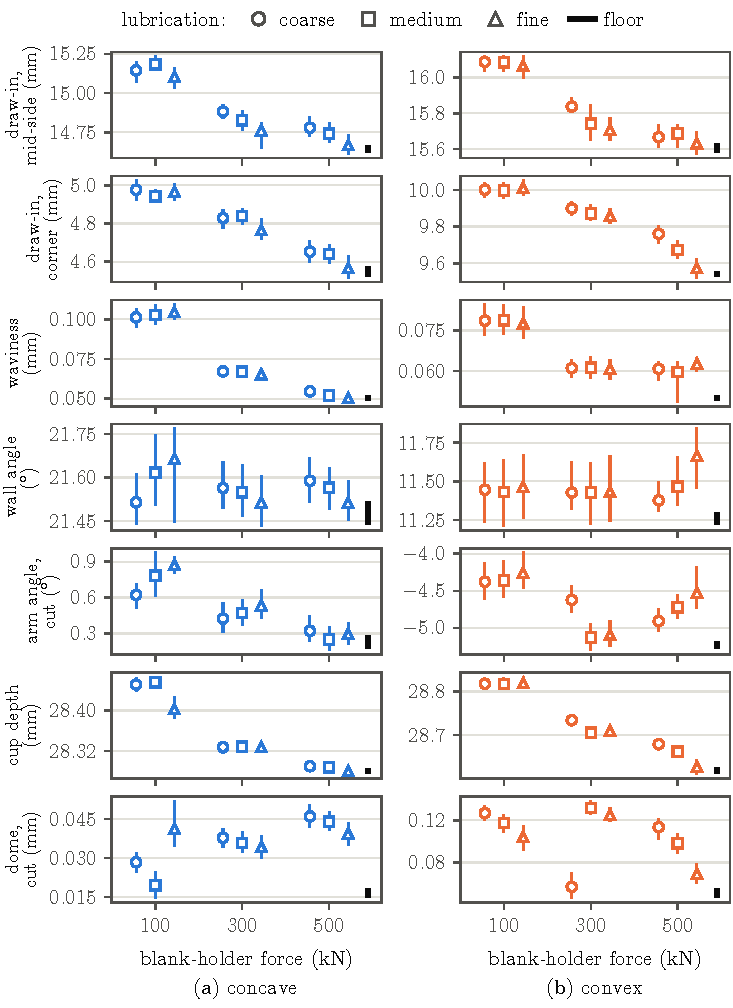
\includegraphics[width=0.82\textwidth]{F1_alternatives}
\caption{Centres of the 18 alternatives (all 500 parts, with 95\,\% intervals over batches) per characteristic and geometry, and one floor (bar)}\label{fig:s-alternatives}
\end{figure}

\begin{figure}[p]
\centering
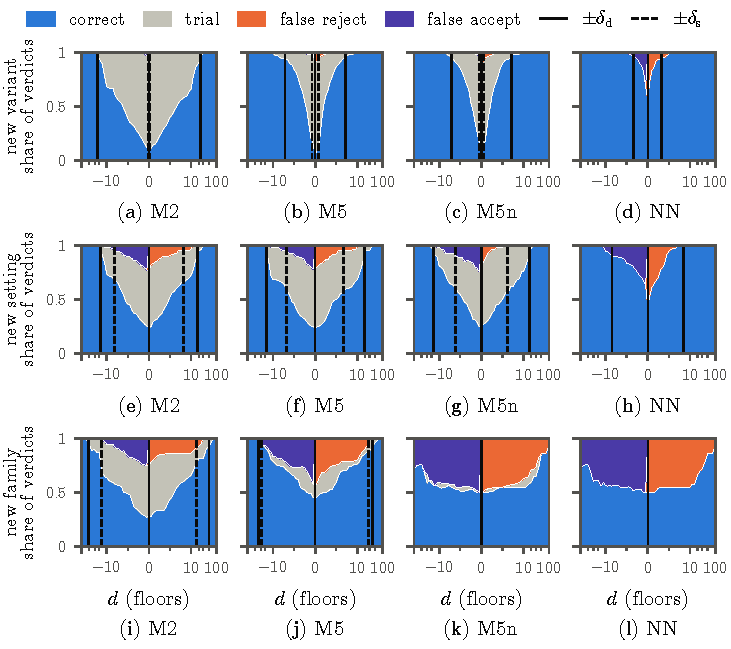
\includegraphics[width=\textwidth]{F3_decisions_compare}
\caption{Verdict shares of M2, M5, M5n and NN against the requirement distance for a new variant, a new setting (pooled) and a new family (produced family's floor)}\label{fig:s-decisions}
\end{figure}

\begin{figure}[p]
\centering
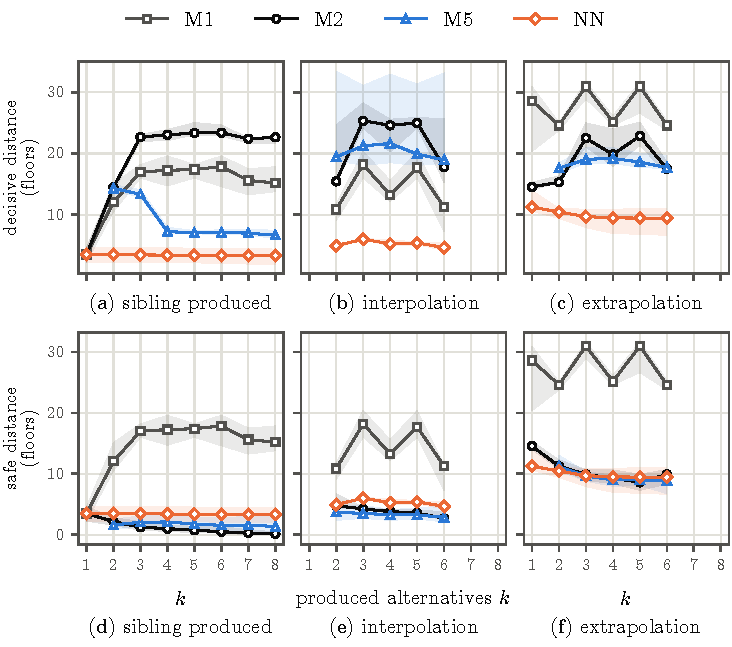
\includegraphics[width=\textwidth]{F4_budget}
\caption{Decisive and safe distances against the number $k$ of produced alternatives, by the relation of the judged design to them; bands: 95\,\% over resamples}\label{fig:s-budget}
\end{figure}

%% BEGIN GENERATED s-coverage
\begin{table}[p]
\tabsizesmall
\setlength{\tabcolsep}{2pt}
\caption{Interval rules: coverage with cluster-bootstrap intervals and interval score by relation}\label{tab:s-coverage}
\begin{tabular}{@{}llrrrrrrrr@{}}
\toprule
 & & \multicolumn{2}{c}{Sibling} & \multicolumn{2}{c}{Interpolated} & \multicolumn{2}{c}{Extrapolated} & \multicolumn{2}{c}{New family} \\
\cmidrule(lr){3-4}\cmidrule(lr){5-6}\cmidrule(lr){7-8}\cmidrule(lr){9-10}
Rule & Level & Cov & IS & Cov & IS & Cov & IS & Cov & IS \\
\midrule
M2 & 0.78 & 89 (83--94) & 19 & 71 & 27 & 44 & 79 & 47 & 124 \\
M2n & 0.78 & 90 (82--96) & 15 & 93 & 14 & 33 & 59 & 12 & 969 \\
M3 & 0.78 & 96 (94--98) & 21 & 43 & 98 & 43 & 120 & 40 & 134 \\
M3n & 0.78 & 89 (81--95) & 11 & 36 & 65 & 48 & 48 & 7 & 989 \\
M5 & 0.90 nominal & 86 (75--94) & 10 & 71 & 29 & 46 & 75 & 12 & 188 \\
M5n & 0.90 nominal & 85 (76--93) & 9 & 93 & 16 & 36 & 55 & 0 & 1024 \\
M7 & 0.90 nominal & 83 (73--92) & 10 & 57 & 81 & 58 & 147 & 17 & 698 \\
M7n & 0.90 nominal & 85 (75--94) & 10 & 52 & 26 & 56 & 41 & 0 & 1043 \\
Mcd & 0.90 nominal & 83 (72--91) & 10 & 79 & 24 & 67 & 50 & 11 & 139 \\
NN+RM & 0.90 & 84 (74--93) & 11 & 88 & 12 & 93 & 24 & 86 & 362 \\
M1sn+RM & 0.90 & 88 (81--94) & 9 & 88 & 12 & 88 & 19 & 86 & 362 \\
M7n+RM & 0.90 & 91 (86--96) & 11 & 90 & 14 & 89 & 19 & 86 & 363 \\
M6 & 0.90 & 93 (87--98) & 15 & 93 & 38 & 61 & 81 & 32 & 145 \\
NN & point & -- & 24 & -- & 42 & -- & 81 & -- & 1067 \\
M1sn & point & -- & 32 & -- & 42 & -- & 77 & -- & 1067 \\
M1s & point & -- & 43 & -- & 122 & -- & 217 & -- & 860 \\
\botrule
\end{tabular}
\footnotetext{Level: guaranteed (largest residual, jackknife+; with a sibling) or nominal coverage. Cov: coverage (\%), with a sibling with a 95\,\% interval over 2000 resamples of the alternatives within each geometry; for a new setting and a new family the alternatives of one held-out cell or family share their calibration set and are near-replicates, so with 2, 4 and 2 such units no useful interval can be given. IS: mean interval score (Gneiting and Raftery 2007) at $\alpha=0.1$, floors; lower is better; for point rules $20\,|e|$. M6: conformal margin on standardised leave-one-out residuals of the calibration set, guaranteed only under exchangeability with them. A new family in the produced family's floor.}
\end{table}
%% END GENERATED s-coverage

%% BEGIN GENERATED s-coverage-qc
\begin{table}[p]
\tabsizesmall
\setlength{\tabcolsep}{2pt}
\caption{Coverage (\%) of the interval rules per characteristic and decision-time stratum}\label{tab:s-coverage-qc}
\begin{tabular}{@{}llrrrrrrrrr@{}}
\toprule
Relation & Rule & Mid-side & Corner & Wavin. & Wall & Arm & Depth & Dome & Not res. & Res. \\
\midrule
sibling & M5 & 89 & 89 & 89 & 83 & 83 & 83 & 83 & 89 & 80 \\
 & \quad interval & 72--100 & 72--100 & 72--100 & 67--100 & 67--100 & 67--100 & 67--100 & 80--97 & 67--95 \\
 & M5n & 89 & 83 & 89 & 72 & 89 & 89 & 83 & 88 & 80 \\
 & \quad interval & 72--100 & 67--100 & 72--100 & 50--89 & 72--100 & 72--100 & 67--100 & 79--96 & 67--93 \\
 & M7n & 83 & 89 & 100 & 89 & 72 & 83 & 78 & 89 & 78 \\
 & \quad interval & 67--100 & 72--100 & 100--100 & 72--100 & 50--89 & 67--100 & 56--94 & 80--97 & 65--93 \\
 & M3 & 100 & 100 & 100 & 89 & 94 & 94 & 94 & 96 & 96 \\
 & \quad interval & 100--100 & 100--100 & 100--100 & 72--100 & 83--100 & 83--100 & 83--100 & 92--100 & 91--100 \\
 & NN+RM & 100 & 89 & 100 & 89 & 72 & 78 & 61 & 95 & 69 \\
 & \quad interval & 100--100 & 72--100 & 100--100 & 78--100 & 56--89 & 61--94 & 39--78 & 87--100 & 52--88 \\
interpolation & M5 & 100 & 100 & 50 & 50 & 100 & 67 & 33 & -- & -- \\
 & M5n & 100 & 100 & 100 & 100 & 67 & 100 & 83 & -- & -- \\
 & M7n & 17 & 100 & 0 & 100 & 67 & 33 & 50 & -- & -- \\
 & M3 & 0 & 67 & 67 & 67 & 50 & 17 & 33 & -- & -- \\
 & NN+RM & 100 & 100 & 67 & 100 & 67 & 100 & 83 & -- & -- \\
extrapolation & M5 & 0 & 50 & 50 & 50 & 58 & 50 & 67 & -- & -- \\
 & M5n & 33 & 0 & 33 & 67 & 25 & 17 & 75 & -- & -- \\
 & M7n & 33 & 92 & 0 & 67 & 92 & 17 & 92 & -- & -- \\
 & M3 & 17 & 17 & 50 & 42 & 67 & 25 & 83 & -- & -- \\
 & NN+RM & 100 & 100 & 75 & 100 & 100 & 75 & 100 & -- & -- \\
\botrule
\end{tabular}
\footnotetext{18 cases per characteristic with a sibling, 6 interpolated, 12 extrapolated. Not res., Res.: the produced siblings do not or do differ resolvably from each other (75 and 51 cases). Interval: 95\,\% over 2000 resamples of the alternatives within each geometry, given only with a sibling (see Table~\ref{tab:s-coverage}).}
\end{table}
%% END GENERATED s-coverage-qc

%% BEGIN GENERATED s-step6
\begin{table}[p]
\tabsizesmall
\setlength{\tabcolsep}{2.2pt}
\caption{The decision rule of step 6, pooled over the families: band, distances and trial shares}\label{tab:s-step6}
\begin{tabular*}{\textwidth}{@{\extracolsep{\fill}}lrrrrrrrrrrrr@{}}
\toprule
 & \multicolumn{4}{c}{Sibling} & \multicolumn{4}{c}{Interpolated} & \multicolumn{4}{c}{Extrapolated} \\
\cmidrule(lr){2-5}\cmidrule(lr){6-9}\cmidrule(lr){10-13}
Rule & $g$ & $\delta_\mathrm{d}/\delta_\mathrm{s}$ & $T_{10}$ & $T_{20}$ & $g$ & $\delta_\mathrm{d}/\delta_\mathrm{s}$ & $T_{10}$ & $T_{20}$ & $g$ & $\delta_\mathrm{d}/\delta_\mathrm{s}$ & $T_{10}$ & $T_{20}$ \\
\midrule
M1 & none & -- & 100 & 100 & 8.75 & 20/2.1 & 44 & 4 & none & -- & 100 & 100 \\
M1s & 2.0 & 6.9/2.9 & 1 & 0 & none & -- & 100 & 100 & none & -- & 100 & 100 \\
M2 & 0 & 23/$<$1 & 33 & 8 & 0.75 & 19/2.0 & 31 & 4 & none & -- & 100 & 100 \\
M5 & 0 & 7.2/$<$1 & 1 & 0 & 0.5 & 20/2.3 & 40 & 4 & none & -- & 100 & 100 \\
M5n & 0 & 7.2/$<$1 & 0 & 0 & 0 & 16/$<$1 & 25 & 0 & 6.75 & 25/1.9 & 48 & 15 \\
NN & 0.25 & 3.6/3.1 & 0 & 0 & 2.0 & 6.7/2.7 & 0 & 0 & 7.0 & 17/2.5 & 26 & 1 \\
M3 & 0 & 23/$<$1 & 45 & 6 & 17.75 & 47/$<$1 & 94 & 69 & 16.75 & 51/$<$1 & 85 & 69 \\
M3n & 0 & 11/$<$1 & 9 & 0 & 6.0 & 21/1.0 & 55 & 6 & 6.5 & 19/1.3 & 47 & 3 \\
M1sn & 0.75 & 4.3/2.8 & 0 & 0 & 2.0 & 6.7/2.7 & 0 & 0 & 6.0 & 15/2.9 & 21 & 0 \\
\botrule
\end{tabular*}
\footnotetext{$g$: guard band (floors) under the reference prior; $\delta_\mathrm{d}/\delta_\mathrm{s}$: distances of the rule with its interval widened by $g$; $T_{10}$, $T_{20}$: share of verdicts sent to trial (\%) at requirements 10 and 20 floors from the truth. None: no band up to 20 floors reaches 95\,\%; so also M0 and M0w in every relation and every rule for a new family.}
\end{table}
%% END GENERATED s-step6

%% BEGIN GENERATED s-guard-family
\begin{table}[p]
\tabsizesmall
\setlength{\tabcolsep}{3pt}
\caption{Guard bands estimated per family and moved between the families}\label{tab:s-guard-family}
\begin{tabular}{@{}llrrrrrrr@{}}
\toprule
 & & & \multicolumn{3}{c}{Concave} & \multicolumn{3}{c}{Convex} \\
\cmidrule(lr){4-6}\cmidrule(lr){7-9}
Relation & Rule & Pooled $g$ & $g$ & Correct & Other $g$ & $g$ & Correct & Other $g$ \\
\midrule
sibling & NN & 0.25 & 0 & 96 & 97 & 0.5 & 96 & 94 \\
 & M1sn & 0.75 & 0.5 & 95 & 97 & 1.0 & 95 & 94 \\
 & M2 & 0 & 0 & 100 & 100 & 0 & 99 & 99 \\
 & M5 & 0 & 0 & 99 & 99 & 0 & 98 & 98 \\
 & M5n & 0 & 0 & 99 & 99 & 0 & 99 & 99 \\
 & M7n & 0 & 0 & 98 & 98 & 0 & 98 & 98 \\
 & Mcd & 0 & 0 & 98 & 98 & 0 & 98 & 98 \\
 & NN+RM & 0 & 0 & 100 & 100 & 0 & 98 & 98 \\
interpolation & NN & 2.0 & 1.5 & 95 & 97 & 2.5 & 95 & 93 \\
 & M1sn & 2.0 & 1.5 & 95 & 97 & 2.5 & 95 & 93 \\
 & M2 & 0.75 & 0.75 & 95 & 95 & 0.5 & 95 & 96 \\
 & M5 & 0.5 & 1.75 & 95 & 91 & 0 & 97 & 99 \\
 & M5n & 0 & 0 & 100 & 100 & 0 & 98 & 98 \\
 & M7n & 0.75 & 0 & 96 & 99 & 1.75 & 95 & 92 \\
 & Mcd & 0 & 0 & 100 & 100 & 1.25 & 96 & 92 \\
 & NN+RM & 0 & 0 & 100 & 100 & 0 & 98 & 98 \\
extrapolation & NN & 7.0 & 9.5 & 95 & 92 & 5.75 & 95 & 100 \\
 & M1sn & 6.0 & 5.5 & 95 & 97 & 6.5 & 95 & 93 \\
 & M2 & none & none & -- & 84 & 6.25 & 95 & -- \\
 & M5 & none & none & -- & 83 & 5.0 & 95 & -- \\
 & M5n & 6.75 & 8.5 & 95 & 92 & 5.0 & 95 & 100 \\
 & M7n & 3.25 & 2.75 & 95 & 98 & 4.75 & 95 & 93 \\
 & Mcd & 6.25 & 8.0 & 95 & 92 & 4.5 & 95 & 99 \\
 & NN+RM & 0 & 0.5 & 95 & 95 & 0 & 100 & 100 \\
new family & NN & none & none & -- & -- & none & -- & -- \\
 & M1sn & none & none & -- & -- & none & -- & -- \\
 & M2 & none & none & -- & -- & none & -- & -- \\
 & M5 & none & none & -- & -- & none & -- & -- \\
 & M5n & none & none & -- & -- & none & -- & -- \\
 & M7n & none & none & -- & -- & none & -- & -- \\
 & Mcd & none & 18.25 & 95 & -- & none & -- & 73 \\
 & NN+RM & none & none & -- & 59 & none & -- & -- \\
\botrule
\end{tabular}
\footnotetext{Reference prior. Correct: share correct among decided verdicts (\%) with the family's own band; Other $g$: with the band of the other family. For a new family, the family is the target of the transfer. None, --: every design to trial.}
\end{table}
%% END GENERATED s-guard-family

%% BEGIN GENERATED s-guard-oos
\begin{table}[p]
\tabsizesmall
\setlength{\tabcolsep}{1.8pt}
\caption{Guard bands validated out of sample under the reference and the release-like prior}\label{tab:s-guard-oos}
\begin{tabular}{@{}llrrrrrrrr@{}}
\toprule
 & & \multicolumn{2}{c}{In sample} & \multicolumn{2}{c}{LOAO, family} & \multicolumn{2}{c}{LOAO, pooled} & \multicolumn{2}{c}{Force cell out} \\
\cmidrule(lr){3-4}\cmidrule(lr){5-6}\cmidrule(lr){7-8}\cmidrule(lr){9-10}
Prior, relation & Rule & $g$ & Corr. & Corr. & T & Corr. & T & Corr. & T \\
\midrule
reference, sibling & NN & 0.25 & 96 & 95 (94--97) & 2 & 95 (94--97) & 2 &  & \\
 & M1sn & 0.75 & 95 & 95 (94--97) & 7 & 95 (94--97) & 6 &  & \\
 & M2 & 0 & 99 & 99 (98--100) & 54 & 99 (98--100) & 54 &  & \\
 & M5 & 0 & 99 & 99 (98--100) & 23 & 99 (97--100) & 23 &  & \\
 & M7n & 0 & 98 & 98 (97--100) & 19 & 98 (97--100) & 19 &  & \\
 & NN+RM & 0 & 99 & 99 (97--99) & 28 & 99 (97--99) & 28 &  & \\
interpolation & NN & 2.0 & 95 & 95 (94--96) & 17 & 95 (94--96) & 17 & 95 (94--96) & 18 \\
 & M1sn & 2.0 & 95 & 95 (94--96) & 17 & 95 (94--96) & 17 & 95 (94--96) & 18 \\
 & M2 & 0.75 & 96 & 95 (95--96) & 52 & 95 (94--96) & 52 & 95 (95--96) & 52 \\
 & M5 & 0.5 & 95 & 96 (96--97) & 56 & 95 (95--96) & 55 & 95 (95--95) & 57 \\
 & M7n & 0.75 & 95 & 95 (95--96) & 28 & 95 (94--96) & 26 & 95 (94--96) & 28 \\
 & NN+RM & 0 & 99 & 99 (99--99) & 42 & 99 (99--99) & 42 & 99 (99--99) & 42 \\
extrapolation & NN & 7.0 & 95 & 94 (92--97) & 56 & 95 (92--98) & 55 & 93 (90--97) & 55 \\
 & M1sn & 6.0 & 95 & 95 (94--96) & 48 & 95 (94--96) & 48 & 95 (94--96) & 48 \\
 & M2 & none & -- & 95 (93--98) & 85 & -- & 100 & 83 (79--87) & 90 \\
 & M5 & none & -- & 95 (92--99) & 82 & -- & 100 & 81 (77--85) & 90 \\
 & M7n & 3.25 & 95 & 95 (93--96) & 58 & 95 (94--96) & 57 & 95 (94--96) & 58 \\
 & NN+RM & 0 & 97 & 97 (95--100) & 74 & 97 (95--100) & 72 & 97 (95--100) & 72 \\
release-like, sibling & NN & 2.0 & 95 & 96 (93--98) & 41 & 95 (91--98) & 35 &  & \\
 & M1sn & 2.75 & 96 & 95 (93--97) & 47 & 95 (92--97) & 48 &  & \\
 & M2 & 0 & 97 & 97 (94--99) & 76 & 97 (94--99) & 75 &  & \\
 & M5 & 0 & 96 & 95 (91--100) & 67 & 97 (93--100) & 78 &  & \\
 & M7n & 6.75 & 97 & 84 (83--100) & 91 & 84 (82--100) & 95 &  & \\
 & NN+RM & 0.5 & 95 & 96 (92--100) & 72 & 94 (89--98) & 68 &  & \\
interpolation & NN & 4.25 & 96 & 95 (94--97) & 66 & 95 (94--96) & 68 & 93 (93--94) & 67 \\
 & M1sn & 4.25 & 96 & 95 (94--97) & 66 & 95 (94--96) & 68 & 93 (92--94) & 67 \\
 & M2 & 2.75 & 97 & 96 (93--99) & 83 & 95 (93--96) & 84 & 94 (93--95) & 85 \\
 & M5 & 2.75 & 95 & 95 (93--97) & 83 & 94 (93--95) & 86 & 88 (87--88) & 84 \\
 & M7n & 3.75 & 96 & 95 (93--98) & 73 & 94 (91--98) & 81 & 87 (85--89) & 74 \\
 & NN+RM & 0 & 95 & 96 (95--97) & 78 & 95 (94--96) & 76 & 95 (94--96) & 77 \\
extrapolation & NN & 14.25 & 95 & 95 (90--98) & 90 & 93 (89--100) & 98 & 72 (68--78) & 93 \\
 & M1sn & 8.5 & 96 & 95 (92--98) & 84 & 96 (93--98) & 84 & 96 (92--98) & 85 \\
 & M2 & none & -- & 94 (89--100) & 97 & -- & 100 & 62 (61--66) & 94 \\
 & M5 & none & -- & 94 (90--100) & 97 & -- & 100 & 61 (58--66) & 94 \\
 & M7n & 6.75 & 96 & 94 (90--100) & 89 & 96 (93--99) & 91 & 94 (90--98) & 91 \\
 & NN+RM & 5.25 & 97 & 97 (94--100) & 95 & 93 (89--100) & 98 & 73 (69--84) & 94 \\
\botrule
\end{tabular}
\footnotetext{Corr.: share correct among decided verdicts (\%), with a 95\,\% cluster interval out of sample; T: share sent to trial (\%). LOAO: band estimated without the held-out alternative, within its family or pooled over both; force cell out: without the held-out geometry--force cell.}
\end{table}
%% END GENERATED s-guard-oos

%% BEGIN GENERATED s-prior
\begin{table}[p]
\tabsizesmall
\setlength{\tabcolsep}{3pt}
\caption{Guard band (floors) and trial rate (\%, in brackets) against the half-width of the prior}\label{tab:s-prior}
\begin{tabular}{@{}llrrrrr@{}}
\toprule
Relation & Rule & $\pm3$ & $\pm5$ & $\pm10$ & $\pm20$ & $\pm50$ \\
\midrule
sibling & NN & 8.0 (99) & 2.0 (37) & 0.5 (5) & 0.25 (2) & 0 (0) \\
 & M1sn & 4.5 (89) & 2.75 (50) & 1.0 (10) & 0.75 (7) & 0.5 (4) \\
 & M2 & 0.5 (85) & 0 (75) & 0 (60) & 0 (54) & 0 (48) \\
 & M5 & 6.5 (99) & 0 (45) & 0 (26) & 0 (23) & 0 (20) \\
 & M7n & 7.25 (99) & 6.75 (99) & 0 (22) & 0 (19) & 0 (17) \\
 & NN+RM & 6.0 (100) & 0.5 (65) & 0 (31) & 0 (28) & 0 (24) \\
interpolation & NN & 5.0 (86) & 4.25 (68) & 2.5 (25) & 2.0 (18) & 1.5 (11) \\
 & M1sn & 5.0 (86) & 4.25 (68) & 2.5 (25) & 2.0 (18) & 1.5 (11) \\
 & M2 & 3.25 (89) & 2.75 (84) & 1.25 (62) & 0.75 (53) & 0 (42) \\
 & M5 & 3.5 (91) & 2.75 (86) & 1.0 (62) & 0.5 (54) & 0 (45) \\
 & M7n & 4.75 (93) & 3.75 (82) & 1.25 (36) & 0.75 (27) & 0.25 (20) \\
 & NN+RM & 0.75 (88) & 0 (75) & 0 (48) & 0 (42) & 0 (37) \\
extrapolation & NN & 14.75 (99) & 14.25 (98) & 8.25 (69) & 7.0 (55) & 5.75 (40) \\
 & M1sn & 9.0 (90) & 8.5 (84) & 6.75 (59) & 6.0 (48) & 5.25 (37) \\
 & M2 & none (100) & none (100) & none (100) & none (100) & 18 (83) \\
 & M5 & none (100) & none (100) & none (100) & none (100) & 17.75 (83) \\
 & M7n & 7.25 (94) & 6.75 (91) & 4.25 (68) & 3.25 (56) & 2.25 (44) \\
 & NN+RM & 5.5 (99) & 5.25 (98) & 0 (79) & 0 (72) & 0 (63) \\
\botrule
\end{tabular}
\footnotetext{Prior: the evaluation grid of requirement distances within the half-width, equal weights; $\pm20$ is the reference prior and $\pm5$ the release-like one. No rule qualifies for a new family.}
\end{table}
%% END GENERATED s-prior

%% BEGIN GENERATED s-guard-qc
\begin{table}[p]
\tabsizesmall
\setlength{\tabcolsep}{1.6pt}
\caption{Share correct (\%) per characteristic with the pooled band, and bands per class of characteristic}\label{tab:s-guard-qc}
\begin{tabular}{@{}llrrrrrrrrrrr@{}}
\toprule
Relation & Rule & $g$ & Mid-side & Corner & Wavin. & Wall & Arm & Depth & Dome & $g_\mathrm{P}$ & $g_\mathrm{G}$ & $g_\mathrm{C}$ \\
\midrule
sibling & NN & 0.25 & 97 & 96 & 99 & 97 & 94 & 96 & 89 & 0 & 0 & 1.75 \\
 & M1sn & 0.75 & 98 & 97 & 93 & 98 & 95 & 93 & 92 & 0.5 & 0.5 & 1.5 \\
 & M2 & 0 & 100 & 99 & 99 & 99 & 100 & 99 & 98 & 0 & 0 & 0 \\
 & M5 & 0 & 100 & 99 & 100 & 99 & 99 & 98 & 94 & 0 & 0 & 0 \\
 & M7n & 0 & 99 & 99 & 100 & 100 & 98 & 98 & 92 & 0 & 0 & 0 \\
interpolation & NN & 2.0 & 97 & 100 & 88 & 100 & 93 & 92 & 96 & 2.0 & 1.5 & 2.5 \\
 & M1sn & 2.0 & 97 & 100 & 88 & 100 & 93 & 92 & 96 & 2.0 & 1.5 & 2.5 \\
 & M2 & 0.75 & 100 & 100 & 90 & 95 & 100 & 99 & 88 & 0 & 0.25 & 1.5 \\
 & M5 & 0.5 & 100 & 100 & 99 & 94 & 100 & 94 & 83 & 0 & 1.0 & 2.5 \\
 & M7n & 0.75 & 97 & 100 & 89 & 100 & 92 & 96 & 93 & 0.75 & 0 & 2.75 \\
extrapolation & NN & 7.0 & 100 & 98 & 89 & 100 & 100 & 86 & 100 & 7.0 & 11.25 & 2.5 \\
 & M1sn & 6.0 & 100 & 100 & 88 & 100 & 90 & 91 & 100 & 6.0 & 6.0 & 6.25 \\
 & M7n & 3.25 & 100 & 100 & 83 & 100 & 100 & 94 & 100 & 4.5 & 1.25 & 0 \\
\botrule
\end{tabular}
\footnotetext{Reference prior. $g_\mathrm{P}$, $g_\mathrm{G}$, $g_\mathrm{C}$: bands estimated for the process indicators (draw-ins, waviness), the drawn geometry (wall angle, depth) and the cut part (arm, dome).}
\end{table}
%% END GENERATED s-guard-qc

\begin{figure}[p]
\centering
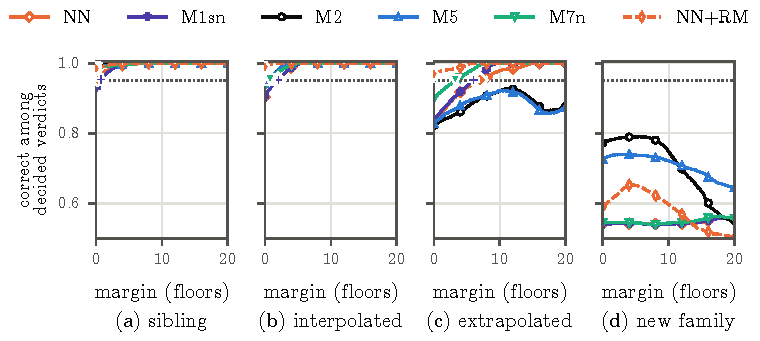
\includegraphics[width=\textwidth]{F5_reliability}
\caption{Share correct among decided verdicts whose margin is at least the value on the axis, reference prior; markers: the guard band $g$ where one qualifies}\label{fig:s-reliability}
\end{figure}

%% BEGIN GENERATED s-costs
\begin{table}[p]
\tabsizesmall
\setlength{\tabcolsep}{3pt}
\caption{Cheapest rule and its expected cost per verdict, with the cost-minimising band of NN}\label{tab:s-costs}
\begin{tabular}{@{}rrrrrr@{}}
\toprule
$c_\mathrm{FR}$ & $c_\mathrm{T}=0.02$ & 0.05 & 0.1 & 0.2 & 0.5 \\
\midrule
\multicolumn{6}{@{}l}{\emph{Sibling}} \\
0.25 & M1sn 0.008 (3.5) & M7n 0.015 (2.0) & NN 0.022 (1.0) & NN 0.027 (0.5) & NN 0.028 (0) \\
0.5 & M1sn 0.009 (4.5) & M7n 0.018 (2.5) & NN 0.026 (1.5) & NN 0.033 (0.5) & NN 0.036 (0) \\
1 & M1sn 0.009 (5.0) & M1sn 0.020 (3.0) & NN 0.031 (2.0) & NN 0.042 (1.0) & NN 0.051 (0) \\
\multicolumn{6}{@{}l}{\emph{Interpolation}} \\
0.25 & NN 0.009 (5.0) & NN 0.022 (4.0) & NN 0.033 (1.5) & NN 0.039 (0.25) & NN 0.040 (0) \\
0.5 & NN 0.010 (5.0) & NN 0.022 (4.5) & NN 0.039 (3.0) & NN 0.054 (1.0) & NN 0.059 (0) \\
1 & NN 0.010 (5.5) & NN 0.023 (5.0) & NN 0.043 (4.5) & NN 0.074 (3.0) & NN 0.096 (0) \\
\multicolumn{6}{@{}l}{\emph{Extrapolation}} \\
0.25 & M1sn 0.014 (14.75) & M1sn 0.034 (10) & M1sn 0.066 (8.25) & NN 0.108 (2.5) & NN 0.117 (0) \\
0.5 & M1sn 0.014 (14.75) & M1sn 0.034 (10) & M1sn 0.067 (8.25) & M1sn 0.113 (3.0) & NN 0.135 (0) \\
1 & M1sn 0.014 (14.75) & M1sn 0.035 (10) & M1sn 0.067 (8.25) & M1sn 0.119 (4.5) & M1sn 0.164 (0) \\
\multicolumn{6}{@{}l}{\emph{New family}} \\
0.25 & trial & trial & M3 0.098 (T) & M2 0.170 (T) & M5 0.215 (0) \\
0.5 & trial & trial & trial & M2 0.183 (T) & M5 0.244 (0) \\
1 & trial & trial & trial & M5 0.198 (T) & M5 0.303 (0) \\
\botrule
\end{tabular}
\footnotetext{Costs relative to a false accept; reference prior; each rule with its cost-minimising band (0 to 40 floors). Trial: sending every design to trial (cost $c_\mathrm{T}$) is cheapest. In brackets: the cost-minimising band of NN (floors); T: NN is cheapest sending every design to trial.}
\end{table}
%% END GENERATED s-costs

%% BEGIN GENERATED s-between
\begin{table}[p]
\tabsizesmall
\setlength{\tabcolsep}{3pt}
\caption{Decisive distance and guard band (floors, in brackets) with a between-run component added to the truths}\label{tab:s-between}
\begin{tabular}{@{}llrrrrr@{}}
\toprule
Relation & Rule & $\tau=0$ & 1 & 2 & 3 & bound \\
\midrule
sibling & NN & 3.4 (0.25) & 3.5 (0.5) & 4.5 (1.5) & 5.8 (2.9) & 4.1 (1.0) \\
 & M1sn & 3.5 (0.75) & 3.9 (1.0) & 4.8 (2.0) & 6.1 (3.25) & 4.4 (1.5) \\
 & M1s & 4.9 (2.0) & 5.6 (2.25) & 6.2 (3.0) & 7.1 (4.25) & 6.1 (3.0) \\
 & M2 & 23 (0) & 23 (0) & 23 (0) & 23 (0.25) & 23 (0) \\
 & M5 & 7.2 (0) & 7.5 (0) & 8.3 (0) & 9.3 (0.75) & 8.3 (0) \\
 & M7n & 6.8 (0) & 7.0 (0) & 7.7 (0) & 8.8 (1.0) & 7.9 (0) \\
& \emph{record rule best} & 100 & 100 & 100 & 100 & 100 \\
interpolation & NN & 4.7 (2.0) & 5.0 (2.25) & 5.5 (3.0) & 6.6 (4.0) & 5.1 (2.75) \\
 & M1sn & 4.7 (2.0) & 5.0 (2.25) & 5.5 (3.0) & 6.6 (4.0) & 5.1 (2.75) \\
 & M1s & 19 (none) & 20 (none) & 21 (none) & 21 (none) & 19 (none) \\
 & M2 & 18 (0.75) & 18 (0.75) & 19 (1.4) & 20 (2.5) & 19 (1.25) \\
 & M5 & 19 (0.5) & 20 (0.75) & 21 (1.25) & 22 (2.25) & 20 (0.9) \\
 & M7n & 7.4 (0.75) & 7.6 (1.0) & 8.4 (1.5) & 9.5 (2.6) & 8.4 (1.25) \\
& \emph{record rule best} & 100 & 100 & 100 & 100 & 100 \\
extrapolation & NN & 9.5 (7.0) & 9.5 (7.25) & 9.5 (7.9) & 10 (8.9) & 9.7 (7.5) \\
 & M1sn & 8.9 (6.0) & 8.8 (6.25) & 9.2 (6.75) & 9.9 (8.0) & 9.0 (6.5) \\
 & M1s & 19 (none) & 19 (none) & 19 (none) & 18 (none) & 19 (none) \\
 & M2 & 18 (none) & 18 (none) & 18 (none) & 19 (none) & 18 (none) \\
 & M5 & 19 (none) & 19 (none) & 19 (none) & 20 (none) & 19 (none) \\
 & M7n & 15 (3.25) & 15 (3.75) & 16 (4.25) & 16 (5.25) & 16 (3.75) \\
& \emph{record rule best} & 100 & 100 & 100 & 100 & 100 \\
new family & NN & 130 (none) & 131 (none) & 132 (none) & 133 (none) & 131 (none) \\
 & M1sn & 131 (none) & 131 (none) & 132 (none) & 133 (none) & 131 (none) \\
 & M1s & 121 (none) & 121 (none) & 121 (none) & 121 (none) & 121 (none) \\
 & M2 & 41 (none) & 41 (none) & 41 (none) & 41 (none) & 41 (none) \\
 & M5 & 35 (none) & 35 (none) & 35 (none) & 35 (none) & 35 (none) \\
 & M7n & 132 (none) & 132 (none) & 133 (none) & 134 (none) & 132 (none) \\
& \emph{record rule best} & 0 & 0 & 0 & 0 & 0 \\
\botrule
\end{tabular}
\footnotetext{Medians over 200 draws (bands over 50); $\tau$: standard deviation of the component (floors); bound: each characteristic's variation between series, $\tau=1.2$--$9.8/2.77$. Record rule best: share of draws in which NN, M1sn or M1n is the most decisive rule (\%).}
\end{table}
%% END GENERATED s-between

%% BEGIN GENERATED s-crossfit
\begin{table}[p]
\tabsizesmall
\setlength{\tabcolsep}{2.4pt}
\caption{Rules and guard bands selected on one geometry and evaluated on the other}\label{tab:s-crossfit}
\begin{tabular}{@{}llllrrrrr@{}}
\toprule
Relation & Criterion & Selected on & Rule & In sample & Other & $g$ & Corr. & T \\
\midrule
sibling & decisive, all rules & concave & NN & 2.0 & 3.6 & & & \\
sibling & decisive, all rules & convex & NN & 3.6 & 2.0 & & & \\
sibling & decisive, pre-specified & concave & M5 & 6.5 & 8.5 & & & \\
sibling & decisive, pre-specified & convex & M5 & 8.5 & 6.5 & & & \\
sibling & safe, all rules & concave & M1sn+RM & 0 & 0.40 & & & \\
sibling & safe, all rules & convex & M1s+RM & 0 & 1.1 & & & \\
sibling & safe, pre-specified & concave & M3 & 0 & 0 & & & \\
sibling & safe, pre-specified & convex & M3 & 0 & 0 & & & \\
sibling & step 6 & concave & NN & 2.0 & 3.6 & 0 & 94 & 0 \\
sibling & step 6 & convex & NN & 4.1 & 2.5 & 0.5 & 97 & 4 \\
interpolation & decisive, all rules & concave & M1n & 3.6 & 5.8 & & & \\
interpolation & decisive, all rules & convex & M1sn & 5.3 & 4.2 & & & \\
interpolation & decisive, pre-specified & concave & M1 & 12 & 6.8 & & & \\
interpolation & decisive, pre-specified & convex & M1 & 6.8 & 12 & & & \\
interpolation & safe, all rules & concave & M1s+RM & 0 & 18 & & & \\
interpolation & safe, all rules & convex & M3n+RM & 0 & 1.8 & & & \\
interpolation & safe, pre-specified & concave & M2 & 2.6 & 3.7 & & & \\
interpolation & safe, pre-specified & convex & M5 & 1.9 & 3.1 & & & \\
interpolation & step 6 & concave & M1n & 5.1 & 7.3 & 1.5 & 93 & 13 \\
interpolation & step 6 & convex & M1sn & 7.8 & 6.8 & 2.5 & 97 & 22 \\
extrapolation & decisive, all rules & concave & M1sn & 8.7 & 8.9 & & & \\
extrapolation & decisive, all rules & convex & NN & 8.7 & 11 & & & \\
extrapolation & decisive, pre-specified & concave & M3n & 12 & 13 & & & \\
extrapolation & decisive, pre-specified & convex & M3n & 13 & 12 & & & \\
extrapolation & safe, all rules & concave & M1sn+RM & 0 & 0.25 & & & \\
extrapolation & safe, all rules & convex & M1s+RM & 0 & 11 & & & \\
extrapolation & safe, pre-specified & concave & M3n & 9.9 & 5.1 & & & \\
extrapolation & safe, pre-specified & convex & M3n & 5.1 & 9.9 & & & \\
extrapolation & step 6 & concave & M1sn & 14 & 14 & 5.5 & 93 & 43 \\
extrapolation & step 6 & convex & NN & 14 & 17 & 5.75 & 92 & 47 \\
new family & decisive, all rules & concave & Mcd & 29 & 33 & & & \\
new family & decisive, all rules & convex & M1 & 33 & 32 & & & \\
new family & decisive, pre-specified & concave & M1 & 32 & 33 & & & \\
new family & decisive, pre-specified & convex & M1 & 33 & 32 & & & \\
new family & safe, all rules & concave & M5+RM & 0.05 & 0 & & & \\
new family & safe, all rules & convex & M1s+RM & 0 & 5.9 & & & \\
new family & safe, pre-specified & concave & M3 & 18 & 17 & & & \\
new family & safe, pre-specified & convex & M3 & 17 & 18 & & & \\
new family & step 6 & concave & Mcd & 43 & 38 & 18.25 & 73 & 83 \\
new family & step 6 & convex & M5+RM & 59 & 81 & 12 & -- & 100 \\
\botrule
\end{tabular}
\footnotetext{Selection by the smallest decisive or safe distance among all rules or the pre-specified ones, or by the smallest decisive distance of step 6; for a new family, selected on one transfer. Other: the distance on the other geometry. Corr., T: share correct and trial rate (\%) there.}
\end{table}
%% END GENERATED s-crossfit

%% BEGIN GENERATED s-design
\begin{table}[p]
\tabsizesmall
\setlength{\tabcolsep}{2.4pt}
\caption{Design-level verdicts: a design meets only if all seven characteristics meet}\label{tab:s-design}
\begin{tabular}{@{}lrrrrrrrr@{}}
\toprule
 & \multicolumn{2}{c}{Sibling} & \multicolumn{2}{c}{Interpolated} & \multicolumn{2}{c}{Extrapolated} & \multicolumn{2}{c}{New family} \\
\cmidrule(lr){2-3}\cmidrule(lr){4-5}\cmidrule(lr){6-7}\cmidrule(lr){8-9}
Rule & Design & Marginal & Design & Marginal & Design & Marginal & Design & Marginal \\
\midrule
M0 & 115/115 & 108/108 & 115/115 & 109/109 & 115/115 & 106/106 & 120/120 & 104/104 \\
M1s & 7.7/7.7 & 4.9/4.9 & 19/19 & 19/19 & 20/20 & 19/19 & 124/124 & 121/121 \\
M2 & 27/1.4 & 23/0.15 & 26/2.8 & 18/2.7 & 27/11 & 18/9.9 & 43/34 & 41/26 \\
M5 & 11/3.6 & 7.2/0.75 & 34/3.8 & 19/2.8 & 34/11 & 19/8.9 & 39/33 & 35/31 \\
M7n & 11/3.6 & 6.8/0.65 & 9.1/5.2 & 7.4/3.4 & 18/1.8 & 15/5.9 & 170/169 & 132/130 \\
NN & 5.1/5.1 & 3.4/3.4 & 5.3/5.3 & 4.7/4.7 & 9.9/9.9 & 9.5/9.5 & 170/170 & 130/130 \\
M1sn & 4.9/4.9 & 3.5/3.5 & 5.3/5.3 & 4.7/4.7 & 9.5/9.5 & 8.9/8.9 & 170/170 & 131/131 \\
NN+RM & 9.5/2.7 & 6.3/0.85 & 9.7/1.1 & 9.6/0.40 & 21/0 & 20/0 & $\infty$/46 & 293/4.5 \\
M3 & 51/2.2 & 23/0 & 32/19 & 29/13 & 41/20 & 33/17 & 57/40 & 40/17 \\
\botrule
\end{tabular}
\footnotetext{Decisive/safe distances (floors). Design: requirements on every characteristic $\delta$ floors above its truth (adequate design) or one characteristic $\delta$ floors below and the others above (failing design), both sides weighted equally. Marginal: per characteristic, as in the main text.}
\end{table}
%% END GENERATED s-design

%% BEGIN GENERATED s-qc
\begin{table}[p]
\tabsizesmall
\setlength{\tabcolsep}{2pt}
\caption{Decisive/safe distances (floors) per characteristic}\label{tab:s-qc}
\begin{tabular}{@{}llrrrrrrr@{}}
\toprule
Relation & Rule & Mid-side & Corner & Wavin. & Wall & Arm & Depth & Dome \\
\midrule
sibling & M0 & 38 & 115 & 15 & 28 & 34 & 115 & 32 \\
 & M1s & 2.2 & 4.3 & 7.2 & 3.0 & 4.2 & 9.0 & 5.0 \\
 & M2 & 20/$<$1 & 6.1/$<$1 & 23/$<$1 & 9.3/$<$1 & 27/$<$1 & 28/$<$1 & 15/$<$1 \\
 & M5 & 3.4/$<$1 & 5.7/1.5 & 1.9/$<$1 & 4.8/1.8 & 7.2/1.2 & 5.4/$<$1 & 12/5.3 \\
 & M7n & 3.4/$<$1 & 3.6/$<$1 & 2.5/$<$1 & 3.5/$<$1 & 6.8/$<$1 & 5.7/1.4 & 12/6.3 \\
 & NN & 2.0 & 4.5 & $<$1 & 3.4 & 2.8 & 3.3 & 7.0 \\
 & M1sn & 2.6 & 3.5 & 3.6 & 3.0 & 4.6 & 3.8 & 6.0 \\
 & M3 & 26/$<$1 & 14/$<$1 & 21/$<$1 & 51/$<$1 & 25/$<$1 & 26/$<$1 & 36/$<$1 \\
interpolation & M0 & 22 & 109 & 15 & 18 & 27 & 115 & 29 \\
 & M1s & 2.8 & 1.3 & 19 & $<$1 & 31 & 12 & 5.7 \\
 & M2 & 11/$<$1 & 7.1/$<$1 & 16/4.2 & 7.6/2.7 & 26/$<$1 & 14/$<$1 & 18/2.8 \\
 & M5 & 16/$<$1 & 5.1/$<$1 & 19/1.3 & 7.6/3.0 & 34/$<$1 & 17/2.2 & 17/3.8 \\
 & M7n & 4.5/1.9 & 6.9/$<$1 & 6.1/3.8 & 3.9/$<$1 & 7.9/5.2 & 8.1/2.7 & 9.1/5.2 \\
 & NN & 3.8 & 1.9 & 4.8 & $<$1 & 5.9 & 4.4 & 5.3 \\
 & M1sn & 3.8 & 1.9 & 4.8 & $<$1 & 5.9 & 4.4 & 5.3 \\
 & M3 & 23/15 & 21/1.8 & 32/9.0 & 16/7.1 & 26/19 & 19/11 & 31/6.3 \\
extrapolation & M0 & 38 & 115 & 8.6 & 28 & 35 & 109 & 32 \\
 & M1s & 4.0 & 2.9 & 21 & 2.0 & 5.9 & 165 & 15 \\
 & M2 & 18/8.3 & 5.4/2.2 & 16/11 & 6.6/3.2 & 28/8.4 & 15/13 & 18/1.3 \\
 & M5 & 20/6.8 & 5.7/2.0 & 17/11 & 7.1/3.2 & 35/8.4 & 17/13 & 16/2.5 \\
 & M7n & 7.9/3.6 & 12/$<$1 & 11/7.5 & 7.6/$<$1 & 19/$<$1 & 15/7.7 & 16/$<$1 \\
 & NN & 6.5 & 6.7 & 11 & 1.9 & 5.4 & 15 & 4.3 \\
 & M1sn & 5.7 & 2.8 & 9.3 & 1.8 & 9.5 & 9.9 & 3.0 \\
 & M3 & 34/19 & 20/11 & 25/16 & 23/8.1 & 44/20 & 22/13 & 39/3.0 \\
new family & M0 & 40 & 113 & 26 & 29 & 40 & 120 & 33 \\
 & M1s & 15 & 107 & 18 & 125 & 43 & 29 & 23 \\
 & M2 & 20/1.9 & 11/3.4 & 32/9.8 & 10/$<$1 & 46/34 & 25/5.9 & 40/36 \\
 & M5 & 5.5/2.1 & 9.9/3.9 & 22/21 & 7.5/3.1 & 39/32 & 20/15 & 40/37 \\
 & M7n & 21/18 & 170/169 & 12/11 & 131/129 & 48/44 & 48/44 & 33/26 \\
 & NN & 20 & 170 & 12 & 130 & 46 & 46 & 28 \\
 & M1sn & 20 & 170 & 13 & 130 & 47 & 45 & 28 \\
 & M3 & 17/3.2 & 15/6.6 & 32/17 & 31/5.3 & 58/40 & 31/15 & 40/17 \\
\botrule
\end{tabular}
\footnotetext{In the floor of the characteristic's geometry; a new family in the produced family's floor. 18 cases per characteristic with a sibling and for a new family, 6 interpolated, 12 extrapolated.}
\end{table}
%% END GENERATED s-qc

%% BEGIN GENERATED s-fewshot
\begin{table}[p]
\tabsizesmall
\setlength{\tabcolsep}{3pt}
\caption{Few-shot transfer to a new family with k produced alternatives of the target family}\label{tab:s-fewshot}
\begin{tabular}{@{}rlrrrrrr@{}}
\toprule
$k$ & Relation & Cases & NN in family & Shifted record & ICM & ICM+sim & Cov ICM \\
\midrule
1 & all & 1008 & 11 & 8.9 & 17/1.6 & 27/1.2 & 85 \\
 & sibling & 252 & 3.5 & 4.8 & 13/0 & 13/0 & 92 \\
 & extrapolation & 756 & 11 & 9.6 & 21/2.5 & 28/2.6 & 83 \\
2 & all & 3528 & 7.7 & 7.8 & 14/1.3 & 19/1.3 & 83 \\
 & sibling & 1638 & 3.5 & 5.9 & 12/0.10 & 13/0.05 & 89 \\
 & interpolation & 378 & 5.0 & 5.8 & 13/1.3 & 15/3.8 & 78 \\
 & extrapolation & 1512 & 10 & 9.5 & 16/3.1 & 24/3.4 & 78 \\
3 & all & 7056 & 5.9 & 8.3 & 13/1.4 & 15/1.3 & 80 \\
 & sibling & 4536 & 3.5 & 7.9 & 11/0.50 & 12/0.30 & 83 \\
 & interpolation & 756 & 6.0 & 8.2 & 13/1.9 & 15/4.1 & 73 \\
 & extrapolation & 1764 & 9.7 & 9.6 & 16/4.0 & 21/3.7 & 75 \\
\botrule
\end{tabular}
\footnotetext{Decisive (and safe) distances in the target family's floor over every subset of $k$ produced alternatives; relation of the judged alternative to the $k$. NN in family: nearest produced setting among the $k$; shifted record: the other family's $q_p$ at the same setting plus the median offset of the $k$; ICM: two-task GP with family intercepts and a free inter-family correlation; ICM+sim: with the nominal simulation in the mean. Cov: coverage of the ICM interval (\%).}
\end{table}
%% END GENERATED s-fewshot

%% BEGIN GENERATED s-paired
\begin{table}[p]
\tabsizesmall
\setlength{\tabcolsep}{3pt}
\caption{Paired differences of the distances between rules, their resolution and the decomposition}\label{tab:s-paired}
\begin{tabular}{@{}llrrr@{}}
\toprule
Pair $a-b$ & & Sibling & Interpolated & Extrapolated \\
\midrule
M5$-$NN & $\delta_\mathrm{d}$ & 3.8 (2.8, 5.2) & 14.4 (13.5, 15.2) & 9.1 (6.9, 12.3) \\
 & $\delta_\mathrm{s}$ & $-$2.6 ($-$3.5, $-$1.6) & $-$1.9 ($-$2.6, $-$1.3) & $-$0.5 ($-$2.5, 2.9) \\
M5n$-$NN & $\delta_\mathrm{d}$ & 3.8 (2.6, 5.1) & 10.9 (10.3, 11.3) & 8.7 (5.6, 11.6) \\
 & $\delta_\mathrm{s}$ & $-$2.8 ($-$3.5, $-$1.7) & $-$4.7 ($-$5.1, $-$4.2) & $-$0.8 ($-$2.4, $-$0.5) \\
M2$-$NN & $\delta_\mathrm{d}$ & 19.3 (17.2, 20.6) & 13.1 (10.4, 13.5) & 8.1 (5.9, 11.4) \\
 & $\delta_\mathrm{s}$ & $-$3.2 ($-$4.4, $-$1.9) & $-$1.9 ($-$2.5, $-$1.5) & 0.5 ($-$2.0, 3.4) \\
M1sn$-$NN & $\delta_\mathrm{d}$ & 0.1 ($-$0.7, 1.4) & 0.0 (0.0, 0.0) & $-$0.6 ($-$1.9, 2.2) \\
 & $\delta_\mathrm{s}$ & 0.1 ($-$0.7, 1.4) & 0.0 (0.0, 0.0) & $-$0.6 ($-$1.9, 2.2) \\
M1s$-$M1sn & $\delta_\mathrm{d}$ & 1.3 (0.7, 3.0) & 14.6 (14.4, 15.1) & 10.3 (5.6, 10.5) \\
 & $\delta_\mathrm{s}$ & 1.3 (0.7, 3.0) & 14.6 (14.4, 15.1) & 10.3 (5.6, 10.5) \\
M5$-$M5n & $\delta_\mathrm{d}$ & 0.0 ($-$0.4, 1.1) & 3.5 (2.9, 4.1) & 0.4 ($-$0.6, 2.2) \\
 & $\delta_\mathrm{s}$ & 0.2 ($-$0.4, 0.6) & 2.8 (2.2, 3.0) & 0.3 ($-$1.8, 4.6) \\
M2$-$M2n & $\delta_\mathrm{d}$ & 3.9 (0.4, 7.3) & 4.4 (2.1, 6.0) & 2.0 ($-$0.2, 3.0) \\
 & $\delta_\mathrm{s}$ & 0.1 ($-$0.5, 0.6) & 2.7 (2.5, 2.8) & 0.8 ($-$1.1, 4.6) \\
M3$-$M3n & $\delta_\mathrm{d}$ & 11.8 (4.4, 15.7) & 14.3 (10.2, 16.2) & 19.8 (11.6, 27.7) \\
 & $\delta_\mathrm{s}$ & $-$0.1 ($-$0.9, 0.1) & 6.3 (2.9, 8.3) & 9.2 (7.1, 12.2) \\
M7n$-$NN & $\delta_\mathrm{d}$ & 3.5 (2.5, 4.8) & 2.8 (2.3, 3.5) & 5.7 (4.2, 8.3) \\
 & $\delta_\mathrm{s}$ & $-$2.7 ($-$3.8, $-$1.5) & $-$1.3 ($-$1.7, $-$1.0) & $-$3.6 ($-$4.5, $-$1.1) \\
M7n$-$M5n & $\delta_\mathrm{d}$ & $-$0.4 ($-$0.9, 0.5) & $-$8.2 ($-$8.6, $-$7.3) & $-$3.0 ($-$3.6, $-$1.0) \\
 & $\delta_\mathrm{s}$ & 0.1 ($-$0.8, 0.8) & 3.4 (2.8, 4.0) & $-$2.8 ($-$3.2, 0.7) \\
M7n$-$M1sn & $\delta_\mathrm{d}$ & 3.3 (2.6, 3.8) & 2.8 (2.3, 3.5) & 6.3 (5.7, 7.0) \\
 & $\delta_\mathrm{s}$ & $-$2.9 ($-$3.5, $-$2.3) & $-$1.3 ($-$1.7, $-$1.0) & $-$3.0 ($-$3.9, $-$1.6) \\
M7$-$M7n & $\delta_\mathrm{d}$ & 0.3 ($-$0.5, 1.1) & 14.7 (13.8, 15.3) & 13.2 (7.9, 39.2) \\
 & $\delta_\mathrm{s}$ & 0.1 ($-$0.2, 0.5) & 12.4 (6.9, 13.3) & 10.7 (3.8, 11.6) \\
NN+RM$-$M5 & $\delta_\mathrm{d}$ & $-$0.9 ($-$1.9, $-$0.3) & $-$9.5 ($-$10.1, $-$8.9) & 1.6 ($-$1.0, 2.6) \\
 & $\delta_\mathrm{s}$ & 0.1 ($-$0.6, 1.1) & $-$2.4 ($-$3.0, $-$1.6) & $-$8.9 ($-$9.8, $-$6.8) \\
NN+RM$-$M7n & $\delta_\mathrm{d}$ & $-$0.5 ($-$1.1, 0.1) & 2.2 (1.4, 2.6) & 5.0 (2.9, 5.5) \\
 & $\delta_\mathrm{s}$ & 0.2 ($-$0.7, 1.4) & $-$3.0 ($-$3.2, $-$2.8) & $-$5.8 ($-$7.3, $-$4.8) \\
Mcd$-$Mc & $\delta_\mathrm{d}$ & $-$19.5 ($-$21.8, $-$16.9) & 7.9 (6.1, 8.7) & $-$15.4 ($-$18.6, $-$7.8) \\
 & $\delta_\mathrm{s}$ & $-$26.2 ($-$28.1, $-$22.7) & $-$12.4 ($-$12.9, $-$11.5) & $-$33.9 ($-$37.3, $-$30.0) \\
\midrule \multicolumn{5}{@{}l}{\emph{Median half-width of the paired 95\,\% intervals (floors)}} \\
point rules & & 2.11 (1.02--2.93) & 0.39 (0.00--0.77) & 2.24 (1.32--3.93) \\
all pairs & & 2.11 (0.75--5.65) & 0.80 (0.00--3.70) & 2.44 (0.85--8.65) \\
\midrule \multicolumn{5}{@{}l}{\emph{Share of the variance of the distances of the pre-specified rules M1--M5}} \\
all relations & $\delta_\mathrm{d}$ & \multicolumn{3}{l}{relation 58\,\%, rule 10\,\%, interaction 32\,\%} \\
within the family & $\delta_\mathrm{d}$ & \multicolumn{3}{l}{relation 16\,\%, rule 60\,\%, interaction 24\,\%} \\
all relations & $\delta_\mathrm{s}$ & \multicolumn{3}{l}{relation 71\,\%, rule 11\,\%, interaction 18\,\%} \\
within the family & $\delta_\mathrm{s}$ & \multicolumn{3}{l}{relation 54\,\%, rule 35\,\%, interaction 11\,\%} \\
\botrule
\end{tabular}
\footnotetext{Difference of rule $a$ minus rule $b$ (floors) with the 95\,\% interval over 1000 common resamples of the held-out alternatives, fits fixed; negative: $a$ closer. Descriptive and not adjusted for the number of comparisons. Decomposition: two-way analysis of the distances of M1--M5 over relations and rules, in the produced family's floor.}
\end{table}
%% END GENERATED s-paired

%% BEGIN GENERATED s-validation
\begin{table}[p]
\tabsizesmall
\setlength{\tabcolsep}{1.8pt}
\caption{The simulation dataset against the measurement per geometry and force}\label{tab:s-validation}
\begin{tabular}{@{}llrrrrlrr@{}}
\toprule
Characteristic & Geometry & kN & Measured & $\mu=0.10$ & Range over $\mu$ & Inside & Closest $\mu$ & Residual \\
\midrule
Draw-in, mid-side & concave & 100 & 15.14 & 16.98 & 16.63--17.34 & no & 0.15 & 30.0 \\
 & concave & 300 & 14.82 & 15.66 & 14.83--16.67 & no & 0.15 & 0.2 \\
 & concave & 500 & 14.73 & 14.85 & 13.59--16.14 & yes & 0.11 & $-$2.4 \\
 & convex & 100 & 16.08 & 18.09 & 17.81--18.41 & no & 0.15 & 33.1 \\
 & convex & 300 & 15.76 & 16.91 & 16.17--17.71 & no & 0.15 & 7.7 \\
 & convex & 500 & 15.66 & 16.05 & 14.78--17.23 & yes & 0.12 & $-$1.7 \\
Draw-in, corner & concave & 100 & 4.962 & 8.385 & 8.240--8.525 & no & 0.15 & 62.2 \\
 & concave & 300 & 4.811 & 7.971 & 7.517--8.328 & no & 0.15 & 51.4 \\
 & concave & 500 & 4.620 & 7.210 & 5.876--8.046 & no & 0.15 & 23.8 \\
 & convex & 100 & 10.00 & 13.48 & 13.31--13.65 & no & 0.15 & 110.5 \\
 & convex & 300 & 9.876 & 13.14 & 12.76--13.47 & no & 0.15 & 96.3 \\
 & convex & 500 & 9.668 & 12.58 & 11.38--13.27 & no & 0.15 & 57.1 \\
Flange waviness & concave & 100 & 0.1028 & 0.08211 & 0.05973--0.09609 & no & 0.05 & $-$1.8 \\
 & concave & 300 & 0.06655 & 0.01440 & 0.01300--0.05128 & no & 0.05 & $-$4.2 \\
 & concave & 500 & 0.05241 & 0.03940 & 0.01075--0.07766 & yes & 0.12 & 0.9 \\
 & convex & 100 & 0.07836 & 0.06604 & 0.05264--0.06648 & no & 0.14 & $-$5.6 \\
 & convex & 300 & 0.06106 & 0.05964 & 0.05690--0.08995 & yes & 0.10 & $-$0.7 \\
 & convex & 500 & 0.06110 & 0.07239 & 0.05734--0.1112 & yes & 0.07 & 1.4 \\
Wall angle & concave & 100 & 21.60 & 20.92 & 19.77--21.10 & no & 0.07 & $-$6.2 \\
 & concave & 300 & 21.54 & 20.32 & 19.44--20.61 & no & 0.11 & $-$11.5 \\
 & concave & 500 & 21.56 & 19.42 & 19.33--20.92 & no & 0.15 & $-$8.0 \\
 & convex & 100 & 11.45 & 10.74 & 10.01--10.91 & no & 0.11 & $-$6.9 \\
 & convex & 300 & 11.43 & 10.30 & 10.30--10.85 & no & 0.05 & $-$7.5 \\
 & convex & 500 & 11.50 & 11.13 & 10.31--11.20 & no & 0.14 & $-$3.9 \\
Arm angle, cut & concave & 100 & 0.7594 & $-$0.4379 & $-$1.103 to 0.1517 & no & 0.05 & $-$5.2 \\
 & concave & 300 & 0.4757 & $-$3.702 & $-$4.363 to $-$1.142 & no & 0.05 & $-$13.9 \\
 & concave & 500 & 0.2892 & $-$4.349 & $-$4.451 to $-$2.928 & no & 0.05 & $-$27.7 \\
 & convex & 100 & $-$4.330 & $-$4.443 & $-$4.687 to $-$3.104 & yes & 0.11 & 0.4 \\
 & convex & 300 & $-$4.947 & $-$5.503 & $-$5.503 to $-$4.246 & yes & 0.06 & 0.0 \\
 & convex & 500 & $-$4.720 & $-$4.296 & $-$5.586 to $-$2.301 & yes & 0.08 & 0.0 \\
Cup depth & concave & 100 & 28.44 & 29.35 & 29.35--29.38 & no & 0.10 & 104.3 \\
 & concave & 300 & 28.33 & 29.34 & 29.31--29.36 & no & 0.06 & 112.1 \\
 & concave & 500 & 28.29 & 29.24 & 29.00--29.33 & no & 0.15 & 82.3 \\
 & convex & 100 & 28.82 & 29.88 & 29.81--29.88 & no & 0.05 & 80.8 \\
 & convex & 300 & 28.72 & 29.64 & 29.47--29.80 & no & 0.15 & 61.5 \\
 & convex & 500 & 28.66 & 29.37 & 29.12--29.64 & no & 0.15 & 37.9 \\
Bottom dome, cut & concave & 100 & 0.02971 & 0.1336 & 0.01244--0.1336 & yes & 0.15 & 0.2 \\
 & concave & 300 & 0.03595 & 0.1387 & 0.03240--0.1753 & yes & 0.15 & $-$1.0 \\
 & concave & 500 & 0.04309 & 0.08286 & $-$0.004812 to 0.1545 & yes & 0.08 & 2.1 \\
 & convex & 100 & 0.1162 & 0.04951 & $-$0.002123 to 0.06661 & no & 0.12 & $-$6.0 \\
 & convex & 300 & 0.1047 & 0.01768 & 0.001869--0.08873 & no & 0.12 & $-$1.9 \\
 & convex & 500 & 0.09375 & 0.02753 & $-$0.0008228 to 0.08175 & no & 0.11 & $-$1.5 \\
\botrule
\end{tabular}
\footnotetext{Values in the unit of the characteristic (signed), simulation at 0.99\,mm. $\mu=0.10$: the nominal simulation; range over $\mu$: over the friction grid 0.05--0.15. Residual: simulation at the closest grid friction minus the measurement (floors). Mc's friction fits end at the upper edge of the grid in 72 of 72 within-family calibrations.}
\end{table}
%% END GENERATED s-validation

%% BEGIN GENERATED s-checks
\begin{table}[p]
\tabsizesmall
\setlength{\tabcolsep}{3pt}
\caption{Checks of the simulation's oil-film mapping, the cup-depth offset and the scanner's lateral scale}\label{tab:s-checks}
\begin{tabular}{@{}llrrrr@{}}
\toprule
Check & Case & a & b & c & d \\
\midrule
oil film & concave, 100\,kN, draw-in, mid-side & 0.89 & $-$0.008 & $-$0.17 & $-$0.37 to +2.00 \\
oil film & concave, 100\,kN, draw-in, corner & 0.36 & 0.035 & 0.15 & 0.11--0.49 \\
oil film & concave, 300\,kN, draw-in, mid-side & 2.30 & 0.091 & 0.36 & 0.25--0.60 \\
oil film & concave, 300\,kN, draw-in, corner & 1.00 & 0.009 & 0.19 & $-$0.04 to +0.67 \\
oil film & concave, 500\,kN, draw-in, mid-side & 3.13 & 0.052 & 0.27 & 0.19--0.34 \\
oil film & concave, 500\,kN, draw-in, corner & 2.69 & 0.050 & 0.20 & 0.06--0.34 \\
oil film & convex, 100\,kN, draw-in, mid-side & 0.77 & 0.029 & 0.05 & 0.02--0.07 \\
oil film & convex, 100\,kN, draw-in, corner & 0.43 & $-$0.018 & $-$0.02 & $-$0.05 to +0.03 \\
oil film & convex, 300\,kN, draw-in, mid-side & 1.93 & 0.069 & 0.39 & 0.35--0.53 \\
oil film & convex, 300\,kN, draw-in, corner & 0.89 & 0.012 & 0.12 & 0.10--0.22 \\
oil film & convex, 500\,kN, draw-in, mid-side & 2.99 & 0.023 & 0.07 & $-$0.08 to +0.23 \\
oil film & convex, 500\,kN, draw-in, corner & 2.29 & 0.010 & 0.39 & 0.35--0.42 \\
\midrule \multicolumn{6}{@{}l}{\emph{Cup depth, flange rise and wall position at 15\,mm depth (mm, simulation at nominal)}} \\
depth & concave, 100\,kN & 0.90 & 0.30 / 0.24 & 2.05 & 0.008 \\
depth & concave, 300\,kN & 1.01 & 0.17 / $-$0.09 & 2.20 & 0.020 \\
depth & concave, 500\,kN & 0.96 & 0.16 / $-$0.29 & 2.02 & 0.039 \\
depth & convex, 100\,kN & 1.06 & 0.15 / 0.09 & 2.16 & 0.006 \\
depth & convex, 300\,kN & 0.92 & 0.12 / 0.03 & 2.08 & 0.053 \\
depth & convex, 500\,kN & 0.70 & 0.14 / 0.05 & 2.06 & 0.006 \\
\midrule \multicolumn{6}{@{}l}{\emph{A dimension fixed by the tooling: cup width at 15\,mm depth}} \\
tooling & concave & $-$0.27 & 0.062 & 0.099 & 0.049 \\
tooling & convex & 0.27 & 0.067 & 0.104 & 0.045 \\
\botrule
\end{tabular}
\footnotetext{Oil film (mm of draw-in per g/m$^2$): a, implied by the dataset's mapping from oil film to friction and the simulated friction sensitivity; b, slope within the run; c, median and d, range of the slopes between the lubrication patterns. Depth: a, simulated minus measured cup depth; b, flange rise towards the edge, measured/simulated; c, wall position at 15\,mm depth, measured minus simulated (radius); d, standard deviation of the press position at bottom dead centre within the series. Tooling: a, correlation of the batch centres of flange width and cup width; b, c, floors of the cup width and of the flange width (mm); d, bound of a lateral scale drift (\%).}
\end{table}
%% END GENERATED s-checks

%% BEGIN GENERATED s-scan
\begin{table}[p]
\tabsizesmall
\setlength{\tabcolsep}{3pt}
\caption{Redundancy of the scans per series, and the components of the floor}\label{tab:s-scan}
\begin{tabular}{@{}lrrrrrr@{}}
\toprule
Series & $W_y-W_x$ & $\sigma_y/\sigma_x$ & $r_{xy}$ & Diagonals & N$-$EW & $r_\mathrm{EW}$ \\
\midrule
concave/100/coarse & 2.49 & 5.9 & 0.01 & 1.84 & 0.12 & 0.09 \\
concave/100/fine & 3.47 & 3.8 & 0.20 & 2.06 & 0.39 & 0.27 \\
concave/100/medium & 2.69 & 6.1 & -0.12 & 1.94 & 0.15 & 0.08 \\
concave/300/coarse & 2.82 & 4.5 & -0.04 & 1.79 & 0.12 & 0.16 \\
concave/300/fine & 2.48 & 4.4 & -0.14 & 1.81 & 0.20 & 0.05 \\
concave/300/medium & 2.70 & 5.8 & 0.06 & 1.75 & 0.12 & 0.17 \\
concave/500/coarse & 3.29 & 4.7 & 0.00 & 1.74 & 0.13 & 0.04 \\
concave/500/fine & 2.86 & 5.1 & -0.01 & 1.64 & -0.05 & -0.10 \\
concave/500/medium & 2.94 & 3.7 & 0.01 & 1.67 & 0.09 & 0.01 \\
convex/100/coarse & 3.46 & 17.7 & 0.05 & 1.94 & -0.92 & -0.66 \\
convex/100/fine & 2.29 & 9.5 & -0.21 & 1.96 & -0.96 & -0.57 \\
convex/100/medium & 2.98 & 16.2 & 0.00 & 1.96 & -0.92 & -0.71 \\
convex/300/coarse & 2.33 & 7.7 & 0.09 & 2.17 & -1.23 & -0.55 \\
convex/300/fine & 2.44 & 7.9 & -0.02 & 1.89 & -0.98 & -0.53 \\
convex/300/medium & 2.43 & 5.3 & 0.01 & 1.87 & -0.92 & -0.54 \\
convex/500/coarse & 2.32 & 5.4 & 0.02 & 2.16 & -1.23 & -0.60 \\
convex/500/fine & 2.40 & 6.1 & -0.00 & 1.96 & -1.64 & -0.62 \\
convex/500/medium & 2.64 & 8.1 & 0.02 & 2.13 & -1.33 & -0.49 \\
\midrule \multicolumn{7}{@{}l}{\emph{Components of the floor, concave/convex}} \\
Draw-in, mid-side & $\sigma_\mathrm{b}/F$ 0.32/0.34 & $\sigma_\mathrm{w}/F$ 0.91/0.66 & drift 3.3 & & & \\
Draw-in, corner & $\sigma_\mathrm{b}/F$ 0.31/0.35 & $\sigma_\mathrm{w}/F$ 0.65/0.77 & drift 4.5 & & & \\
Flange waviness & $\sigma_\mathrm{b}/F$ 0.33/0.30 & $\sigma_\mathrm{w}/F$ 0.55/1.31 & drift 2.5 & & & \\
Wall angle & $\sigma_\mathrm{b}/F$ 0.32/0.26 & $\sigma_\mathrm{w}/F$ 0.68/1.39 & drift 2.1 & & & \\
Arm angle, cut & $\sigma_\mathrm{b}/F$ 0.36/0.31 & $\sigma_\mathrm{w}/F$ 0.46/1.22 & drift 2.6 & & & \\
Cup depth & $\sigma_\mathrm{b}/F$ 0.31/0.34 & $\sigma_\mathrm{w}/F$ 0.65/0.52 & drift 3.9 & & & \\
Bottom dome, cut & $\sigma_\mathrm{b}/F$ 0.33/0.36 & $\sigma_\mathrm{w}/F$ 0.76/0.55 & drift 3.9 & & & \\
\botrule
\end{tabular}
\footnotetext{$W_y-W_x$: flange width in the direction of motion minus that along the laser line (mm); $\sigma_y/\sigma_x$: ratio of their part-to-part standard deviations; $r_{xy}$: their correlation; diagonals: difference of the two flange diagonals (mm); N$-$EW: north wall angle minus the mean of east and west ($^\circ$); $r_\mathrm{EW}$: correlation of east and west. Components: $\sigma_\mathrm{b}$ between batch means, $\sigma_\mathrm{w}$ within batches, drift: floor over that of permuted series.}
\end{table}
%% END GENERATED s-scan

\end{document}
